% NØNOS whitepaper, release 0.9.3.
% Build with tectonic or xelatex:  make -C paper
\documentclass[a4paper,10pt]{article}

\usepackage[a4paper,left=2.4cm,right=2.4cm,top=2.4cm,bottom=2.5cm,footskip=1.1cm]{geometry}
\usepackage{fontspec}
\setmainfont{Geist}[Path=./fonts/,Extension=.ttf,UprightFont=*-Regular,BoldFont=*-SemiBold,
  ItalicFont=*-Medium,BoldItalicFont=*-SemiBold,Mapping=,Ligatures=NoCommon]
\newfontfamily\geistmedium{Geist}[Path=./fonts/,Extension=.ttf,UprightFont=*-Medium,Mapping=,Ligatures=NoCommon]
\setmonofont{JetBrainsMono}[Path=./fonts/,Extension=.ttf,UprightFont=*-Regular,BoldFont=*-Bold,Scale=0.86,Mapping=,Ligatures=NoCommon]

\usepackage{xcolor}
\definecolor{ink}{HTML}{0A0B0D}
\definecolor{teal}{HTML}{007C85}
\definecolor{cyan}{HTML}{66FFFF}
\definecolor{deep}{HTML}{2E5C5C}
\definecolor{paper}{HTML}{F2F3F7}
\definecolor{mute}{HTML}{5B6470}
\definecolor{rule}{HTML}{C9CED6}
\definecolor{refuse}{HTML}{B3261E}

\usepackage{microtype}
\usepackage{graphicx}
\usepackage{tikz}
\usetikzlibrary{arrows.meta,positioning,calc,fit,shapes.misc,backgrounds,decorations.pathreplacing}
\usepackage{booktabs,longtable,array,tabularx}
\usepackage{caption}
\usepackage{titlesec}
\usepackage{enumitem}
\usepackage{fancyhdr}
\usepackage{etoolbox}
\usepackage{footmisc}
\usepackage{float}
\usepackage[hyphens]{url}
\urlstyle{tt}
\def\UrlFont{\ttfamily\footnotesize}

\usepackage[colorlinks=true,linkcolor=teal,urlcolor=teal,citecolor=teal,
  pdftitle={NØNOS: A Computer That Can Prove What It Runs (whitepaper, release 0.9.3)},
  pdfauthor={NØNOS},pdfsubject={Whitepaper on NØNOS release 0.9.3},
  pdfkeywords={microkernel, capabilities, STARK, Wayland, Linux, sandbox}]{hyperref}

% Spacing and shape of the text.
\setlength{\parindent}{0pt}
\setlength{\parskip}{0.55em plus 0.15em minus 0.1em}
\linespread{1.05}
\setlist{nosep,leftmargin=1.4em,itemsep=0.25em}
\emergencystretch=2em
\widowpenalty=10000 \clubpenalty=10000

% Headings: sentence case, semibold, numbered in teal.
\titleformat{\section}{\Large\bfseries\color{ink}}{\color{teal}\thesection}{0.7em}{}
\titlespacing*{\section}{0pt}{2.2em}{0.6em}
\titleformat{\subsection}{\large\bfseries\color{ink}}{\color{teal}\thesubsection}{0.6em}{}
\titlespacing*{\subsection}{0pt}{1.5em}{0.4em}
\titleformat{\subsubsection}{\normalsize\bfseries\color{ink}}{}{0em}{}
\titlespacing*{\subsubsection}{0pt}{1.1em}{0.2em}

% Running head and foot.
\pagestyle{fancy}
\fancyhf{}
\renewcommand{\headrulewidth}{0.3pt}
\renewcommand{\headrule}{\hbox to\headwidth{\color{rule}\leaders\hrule height \headrulewidth\hfill}}
\fancyhead[L]{\footnotesize\color{mute}\texttt{N\O{}NOS}}
\fancyhead[R]{\footnotesize\color{mute}A computer that can prove what it runs}
\fancyfoot[C]{\footnotesize\color{mute}\thepage}
\fancyfoot[R]{\footnotesize\color{mute}\texttt{release 0.9.3}}
\fancypagestyle{plain}{\fancyhf{}\fancyfoot[C]{\footnotesize\color{mute}\thepage}\renewcommand{\headrulewidth}{0pt}}

% Footnotes hold the source citations.
\renewcommand{\footnotesize}{\fontsize{8.4}{10.2}\selectfont}
\setlength{\footnotesep}{0.9em}
\renewcommand{\footnoterule}{\vspace*{-3pt}{\color{rule}\hrule width 0.3\columnwidth height 0.3pt}\vspace*{4pt}}
\newcommand{\src}[1]{\footnote{\path{#1}}}
\newcommand{\srcs}[2]{\footnote{\path{#1}; \path{#2}}}
\newcommand{\srcss}[3]{\footnote{\path{#1}; \path{#2}; \path{#3}}}
\newcommand{\srcsss}[4]{\footnote{\path{#1}; \path{#2}; \path{#3}; \path{#4}}}
\newcommand{\note}[1]{\footnote{#1}}

% Inline code and names.
\newcommand{\code}[1]{\texttt{#1}}
\newcommand{\nonos}{N\O{}NOS}

% Captions.
\captionsetup{font={small,color=ink},labelfont={bf,color=teal},labelsep=period,
  justification=raggedright,singlelinecheck=false,skip=6pt,width=\textwidth}
\setlength{\textfloatsep}{14pt plus 2pt minus 4pt}
\setlength{\floatsep}{12pt plus 2pt minus 2pt}
\renewcommand{\topfraction}{0.9}
\renewcommand{\bottomfraction}{0.8}
\renewcommand{\textfraction}{0.08}
\renewcommand{\floatpagefraction}{0.75}

% Tables.
\renewcommand{\arraystretch}{1.18}
\setlength{\heavyrulewidth}{0.7pt}
\setlength{\lightrulewidth}{0.35pt}

% A call-out for statements of what is not claimed.
\usepackage[breakable,skins]{tcolorbox}
\newtcolorbox{callout}[1][]{enhanced,breakable,colback=paper,colframe=paper,
  borderline west={2pt}{0pt}{teal},boxrule=0pt,arc=0pt,left=9pt,right=8pt,top=6pt,bottom=6pt,
  fontupper=\small,before skip=0.8em,after skip=0.8em,#1}

\newcommand{\nPrograms}{31}
\newcommand{\nWAYLAND}{7}
\newcommand{\nTTY}{24}
\newcommand{\nFILESHOME}{31}
\newcommand{\nEXEC}{8}
\newcommand{\nNETANON}{8}
\newcommand{\nNETLISTENLO}{3}
\newcommand{\nJIT}{1}


\begin{document}
\raggedbottom
\thispagestyle{plain}
\begin{tikzpicture}[remember picture,overlay]
  \fill[ink] (current page.north west) rectangle ([yshift=-8.6cm]current page.north east);
  \fill[teal] ([yshift=-8.6cm]current page.north west) rectangle ([yshift=-8.68cm]current page.north east);
  \node[anchor=north west,inner sep=0pt] at ([xshift=2.5cm,yshift=-1.9cm]current page.north west)
    {
\includegraphics[height=1.15cm]{logo/nonos-logo-cyan.pdf}};
  \node[anchor=north west,text width=15.4cm,inner sep=0pt,text=white] at
    ([xshift=2.5cm,yshift=-3.9cm]current page.north west)
    {\fontsize{25}{29}\selectfont\bfseries A computer that can prove\\what it runs\par
     \vspace{0.9em}
     {\fontsize{12.5}{16}\selectfont\color{cyan}\mdseries Release 0.9.3: proof for the software we ship,\\and a box for everyone else's\par}
     \vspace{1.1em}
     {\footnotesize\ttfamily\color{white!70!ink} whitepaper on release 0.9.3 \quad repository commit \quad 30 October 2026\par}};
\end{tikzpicture}
\vspace*{6.3cm}

{\footnotesize\color{mute}\ttfamily https://nonos.software \quad https://github.com/NON-OS/microkernel-preview \quad https://verify.nonos.software}

\vspace{1.1em}
{\large\bfseries\color{teal} Abstract}\par\vspace{0.2em}
\noindent\nonos{} is an operating system for x86\_64 computers that tries to make its software state checkable, by the machine and by someone else, before that software is trusted with keys, money or traffic. A Rust capability microkernel keeps page tables, scheduling, IPC and 183 checked system calls in ring 0. Drivers, the network stack, the desktop and a wallet run in ring 3 as 152 signed capsules, each admitted at spawn by two signatures and a STARK membership proof under one policy root.

Release 0.9.3 adds what 0.9.2 left open: programs the project did not write. A Linux program opens its own window on the desktop, inside a box named by its signed Marketplace listing: a window, its own home folder, the chosen anonymity network, a terminal, the right to start programs. The program holds no capability of its own. The kernel sends every call it makes to one supervisor capsule, which applies the box, and keeps its own count of the answers. We show what the system refused when single hostile attempts were made from inside a program, and what it did not, and list the three known ways around the box.

The paper says what has been proved, what has been booted, and what is only designed. No independent audit has been done.


\begin{callout}
\textbf{Reading this paper.} Every technical statement cites a file in the repository at the commit above, with line numbers where they help, in a numbered footnote. A claim we could not tie to the tree is not made. Where two documents in the tree disagree, we say so and follow the code. Section~\ref{sec:why} states the problem. Sections~\ref{sec:arch} to~\ref{sec:capsules} describe the kernel and how it admits software. Section~\ref{sec:box} is the centre of this release: running programs we did not write. Section~\ref{sec:status} says what has run and what has not. Nothing in this paper is an audit, and none has been done.
\end{callout}
\clearpage

\section{Why \nonos{} exists}\label{sec:why}

A computer cannot tell anyone, in a form that can be checked, what software it is running. A person who signs a transaction on a laptop trusts that the signing program is the one they meant to run, that no other program can read its key, and that the network path does not give them away. None of this is visible from outside, and little of it is visible from inside.

Public blockchains moved most of the trust in a payment system into code that anyone can check. Ethereum verifies every state transition with rules that every node enforces. The machines at its edges sit outside that system. A wallet key lives on a general-purpose computer with thousands of programs that can read its memory or its disk. A validator signs with keys on a server whose kernel and drivers nobody outside can see. A remote procedure call provider learns the address of every machine that asks it about an account. A mixnet hides traffic patterns only for the traffic that is actually sent through it, and an operating system that lets any program open a direct socket undoes the protection without telling the person.

\nonos{} starts from the endpoint. Release 0.9.2 asked three questions of every piece of code before it runs. Which image is this, and is it one of the images a policy committed to? What may it reach once it runs? Which network carries what it sends? The answers are enforced in a small kernel and, where we could, made checkable by someone who does not trust the machine.

\subsection{The problem 0.9.2 left open}

Those three questions have a quiet assumption in them: that the code is ours. Every one of the 152 capsules in the 0.9.3 tree is built by the project, signed with two algorithms and enrolled under one policy root, so the proof at admission says something exact about it.\note{\path{README.md}, section "Capsules".} A person does not live in a machine like that. They want a password manager somebody else wrote, a chat client, an editor they have used for ten years, a Monero wallet, a PDF viewer. If the system will run only what the project signed, it is a demonstration. If it will run anything, then the proofs describe a small part of what is on the machine, and the rest is as trustworthy as a stranger's download.

Most systems settle this by trusting the program. They check that it came from a store, then give it the person's files, the network and the screen, because it asked for them. A permission dialog is the usual refinement, and it moves the decision to the one party least able to make it. A person cannot read a Qt application's system calls. They can read a short list of what it asks for, if the list is enforced.

\subsection{The thesis}

We make two kinds of statement, and keep them apart.

For software the project ships, \nonos{} makes a statement about \emph{identity}: this exact file, with exactly these rights, is a member of the set one policy root committed to. That is a proof, checked by the kernel at every spawn, and checkable by anyone from outside.

For software the project did not write, an identity proof would say much less, and would be easy to mistake for more. We cannot prove that a Qt application behaves. We can make a statement about \emph{reach}: this program gets a window, a home folder and the Anyone network, and nothing else, and the part of the system that enforces that is small, is itself admitted by proof, and sees every call the program makes. The list is short, it is part of the program's signed Marketplace listing, and a person can read it before they install.

The argument of this paper is that a capability microkernel is the right place to make the second statement. A microkernel has already moved drivers, the network stack and the desktop out of ring 0, so nearly everything a foreign program could want is a message to a small, named capsule with a capability word. The kernel does not need to understand Linux to hold a Linux program to a box. It needs to give the program nothing of its own, send every call to one checker, and keep its own count of what happened. Section~\ref{sec:box} works through that.

The release has a second half to its thesis, which is about honesty. A box is a claim, and claims fail. So the paper reports what the kernel refused when we ran real programs against it, what it did not refuse because the program was granted the right, and which of the ways around the box we already know about.

\subsection{What this paper covers}

Sections~\ref{sec:goals} and~\ref{sec:model} state the goals and the threat model. Sections~\ref{sec:arch} to~\ref{sec:capsules} describe the kernel, the chain of trust and the capsule format, which 0.9.2 introduced and 0.9.3 extends: the tree grew from 91 capsules to 152, and from 18 driver capsules to 67. Section~\ref{sec:box} is the new centre. Sections~\ref{sec:crypto} to~\ref{sec:verify} cover cryptography, networking and verification. Section~\ref{sec:eth} keeps the 0.9.2 discussion of Ethereum as a direction, with what changed. Sections~\ref{sec:status} to~\ref{sec:next} give the status of each component, use cases, limitations and the work we have not done. Section~\ref{sec:related} places the design among its neighbours.

\section{Design goals}\label{sec:goals}

The project writes its rules in \code{docs/overview/design-principles.md} and \code{docs/overview/mission.md}. We restate them as eight goals, say where each is enforced, and say which of them 0.9.3 changes. A goal is only useful if a reader can find the code that holds it, so each one points at a file.

\textbf{G1. Least privilege by capability word.} Every process holds a mask over 40 capability bits, fixed from its signed manifest at spawn, and every system call is checked against it. In 0.9.2 the mask had 36 bits. The four added since are \code{InputConsumer}, \code{CameraCapture}, \code{MicrophoneCapture} and \code{ScreenCapture}.\srcs{src/capabilities/types/defs.rs:17-76}{src/syscall/contract/dispatch.rs:31-45}

\textbf{G2. Everything that runs is signed and measured.} The loader checks the kernel. The kernel checks the loader and every capsule. Admission needs two signature algorithms and a STARK membership proof.\src{docs/security/boot-chain-and-signatures.md}

\textbf{G3. The verifier is on the machine, the prover is elsewhere.} The kernel and the loader link only \code{nox\_verify}. Proofs are made on the enrolling host by \code{nonos-stark-enroll}.\srcs{Cargo.toml:1444}{nonos-stark-enroll/Cargo.toml:15-19}

\textbf{G4. Drivers run in ring 3.} A driver is a capsule that reaches hardware only through grants from the kernel's broker, with DMA confined by the IOMMU where a remapping unit is in service. There are 67 driver capsules in 0.9.3.\src{docs/overview/architecture-hardware-broker-iommu.md}

\textbf{G5. Amnesic by default.} A boot keeps nothing unless the person installs, and an orderly power-off wipes memory first. In 0.9.3 the desktop's Power Off item and the Power key both run that wipe.\srcs{nonos.toml:25-28}{src/security/zerostate/terminate.rs:23-45}

\textbf{G6. Refuse rather than fall back.} A chosen anonymity network that is not running means no route. Nothing is retried in the clear.\src{userland/nonos_route_link/src/pick.rs:130-139}

\textbf{G7. Proofs sit next to the code.} Host proof crates compile the shipped source through \code{\#[path]}, and Lean 4 models state the properties the code owes.\src{verification/lean/REFINEMENT.md}

\textbf{G8 (new in 0.9.3). A foreign program holds nothing of its own.} A Linux program is a process with an empty capability word. Everything it can do, it does through a supervisor that holds a box, and the box is part of the program's signed listing.\srcs{src/process/foreign/spawn_guest.rs:41-48}{userland/nonos_linux_policy/README.md:1-12}

The project also says what it does not claim: functional correctness of the whole kernel, hardware breadth, anonymity against every observer, and an independent audit.\note{\path{docs/overview/mission.md}, section "What NONOS is not".} We add one. G8 is a goal, not a result. Section~\ref{sec:box} says how far the evidence goes.

\section{System and threat model}\label{sec:model}

\subsection{System model}

The machine is an x86\_64 computer with UEFI firmware, optionally a TPM 2.0, and optionally an Intel VT-d or AMD-Vi remapping unit. The loader \code{BOOTX64.EFI} starts the kernel. The kernel starts its capsules from the kernel image and from a signed store. A build is one of seven profiles: standard, hardened, airgapped, qemu, dev, selftest and core. A release image is built hardened, which requires Secure Boot and a TPM at boot.\note{\path{README.md}, section "Build it"; \path{docs/build/profiles.md}.}

\subsection{Assets}

The threat model lists what it protects and what guards each asset.\src{docs/overview/threat-model-assets.md} Five matter here. The wallet's key, held by the keyring capsule. The record of what runs, held by signatures, attestation and the capability word. The device secret, derived from the TPM and released to one capsule. The data volume, sealed under a key the TPM derives from the current boot state. And, new in 0.9.3, the person's own files and the contents of other programs' memory, which a Linux program must not reach unless its listing says it may.

\subsection{Adversaries in scope}

\begin{itemize}
\item A capsule, an app or a Linux program that tries to reach past its capability word or its box.
\item A device that attempts DMA outside its capsule's grants, where a remapping unit in service covers it.
\item An observer on the network path, for connections made under Nym or Anyone.
\item Someone who reads the disk of a machine that is off.
\item A capsule or kernel changed after it was signed and enrolled; a loader changed after enrolment that still hands the kernel the TPM event log; an older signed kernel put back on a machine whose TPM holds the rollback floor.
\end{itemize}

This is the project's own list.\src{docs/overview/threat-model-in-scope.md} The first item is the one 0.9.3 widens. The Linux programs we have in mind are not hostile by default. A KeePassXC build from a distribution is probably fine. But the point of a box is that nobody has to decide that, and the adversary we design against is a program that behaves as a hostile one would: reads the person's files, signals other programs, opens a socket to somewhere it was not told about, starts a tool it was not given. We also design against the plainer case, a bug in a program that a hostile document can steer.

What a hostile Linux program gets is spelled out in the threat model. It holds no capabilities. The kernel parks each of its Linux system calls for the personality to answer, and refuses every native call except \code{MkTtyQuery}, which only describes the caller's own streams. The personality's ordinary run and terminal instances hold no Network capability, and every network service requires it.\note{\path{docs/overview/threat-model-assets.md}, section "A hostile Linux program"; \path{src/process/foreign/trap.rs:28-57}; \path{src/syscall/contract/cap_table/mk_surface.rs:60}.}

The threat model also says the personality is itself a capsule, so a program that subverts it gets the personality's bits and no more. Those are CoreExec, IPC, Memory, Crypto, FileSystem, Debug, two display bits, StoreWrite, ForeignExec and LocalSign, with Network added in the install role.\srcs{userland/capsule_linux/Capsule.mk:50-59}{src/userspace/capsule_linux/spawn.rs:39-55} That is a long list, and it is the honest answer to "how strong is the box": as strong as the supervisor that enforces it, plus the kernel's refusal to let a guest do anything on its own. Section~\ref{sec:box-limits} comes back to this.

\subsection{Assumptions and exclusions}

\nonos{} trusts the CPU, the UEFI firmware until \code{ExitBootServices}, and the TPM. It assumes the IOMMU translates as its tables say, RDRAND and RDSEED are unpredictable, BLAKE3, SHA-2, SHA-3 and the width-8 Poseidon hash are collision resistant, and the Rust compiler is correct.\note{\path{docs/overview/threat-model-a-tampered-image.md}, section "Assumptions".} Out of scope are lying firmware or TPMs; physical access to a running machine; DMA from a device that no remapping unit covers; timing and cache side channels between capsules; a kernel panic, which wipes the kernel heap and powers off but not process memory; and a power cut, which wipes nothing.\srcs{docs/overview/threat-model-in-scope.md}{docs/release/0.9.3-security-limits.md}

Without a TPM, the rollback floor is absent in every boot mode except Hardened and Air-Gapped, and the kernel's check of its loader rests on the loader's own word.\src{docs/security/protections-and-limits-what-nonos-does.md}

Compared with 0.9.2, two exclusions moved. AMD-Vi is now driven in every build profile, so "every device on AMD-Vi platforms" is no longer outside the model, although it has run only under QEMU's AMD IOMMU and not on an AMD machine. And on a machine whose firmware left the remapping unit off, a Standard boot now says so on its \code{[IOMMU]} line, in the attestation, on the splash and in About, and Hardened and Air-Gapped stop instead.\srcs{docs/release/0.9.3-supported-hardware.md}{docs/release/0.9.3-security-limits.md}

\section{Architecture}\label{sec:arch}

\subsection{What stays in ring 0}

The kernel is written in Rust. At the commit studied, \code{src/} holds 7,579 Rust files and 389,695 lines (our count, with \code{git ls-tree} and \code{wc}; the README says about 390,000). In 0.9.2 the same count gave 5,139 files. We have not measured where the growth sits. What we can say is what ring 0 still keeps: only address spaces and page tables, the scheduler with symmetric multiprocessing up to 256 CPUs, IPC, capabilities, the system-call boundary, process creation and the capsule spawn gate. It also keeps the TPM driver and the encrypted data volume, a hardware broker that hands device windows to driver capsules, and the kernel's record of what each Linux guest did (Section~\ref{sec:box}).\srcs{src/smp/constants.rs:17}{docs/overview/architecture-kernel-in-ring.md}

Everything else runs in ring 3. The tree has 152 directories with a \code{Capsule.mk}, up from 91 at the 0.9.2 changelog, and 67 of them are driver capsules, up from 18 (Table~\ref{tab:counts}). Figure~\ref{fig:layers} shows the split.

\begin{figure}[t]
\centering
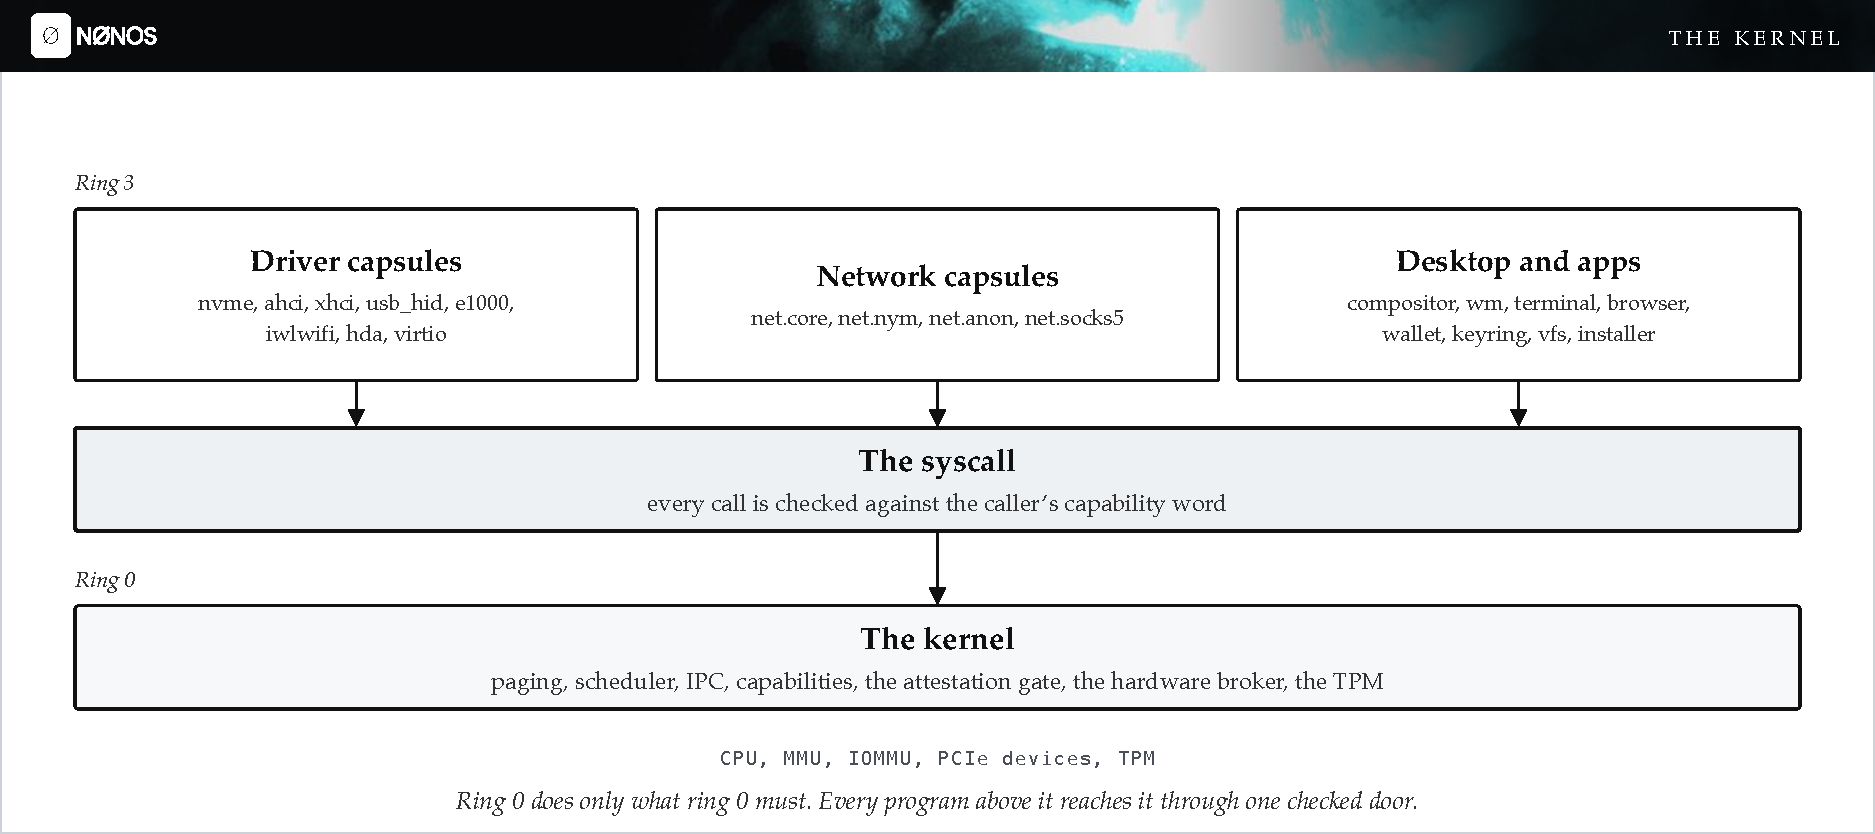
\includegraphics[width=0.84\textwidth]{figures/diagram-layers.pdf}
\caption{The kernel and everything above it. Ring 3 holds drivers, network services, the desktop and every program; ring 0 holds what only ring 0 can do. Every program reaches the kernel through one checked door, the system call. Drawn from \code{docs/overview/architecture.md} and the capsule list in the tree.}
\label{fig:layers}
\end{figure}

\begin{table}[t]
\centering
\caption{What grew between the 0.9.2 changelog and the 0.9.3 tree. Counted from git at the commit where \code{CHANGELOG-0.9.2.md} landed (6 October 2026) and at the studied commit. About 6,000 commits separate them. Capsules are directories with a \code{Capsule.mk}; proof crates are directories ending in \code{\_proofs} with a \code{Cargo.toml}.}
\label{tab:counts}
\begin{tabular}{@{}lrr@{}}
\toprule
 & 0.9.2 & 0.9.3\\ \midrule
Driver capsules & 18 & 67\\
Capsules in all & 91 & 152\\
Rust files in the kernel, \code{src/} & 5,139 & 7,579\\
Rust files in \code{userland/} & 10,069 & 31,674\\
Proof crates & 56 & 223\\
System calls & 130 & 183\\
Capability bits & 36 & 40\\ \bottomrule
\end{tabular}
\end{table}

The first four rows are the project's counts and we reproduced them from the git trees. The last two come from the ABI files, which a checker holds to the kernel.\srcs{abi/syscalls.toml}{scripts/check_syscall_abi.py} Run on this tree, the checker reports "183 published syscalls reach a handler" and \code{check\_caps\_abi.py} reports "40 published bits agree with the kernel". A word on the 0.9.2 figures: that paper counted at a later commit than the changelog, and its own count of kernel files was 5,758. We use the changelog commit for both columns so that the comparison is of like with like.

\subsection{The system-call ABI}

A call number is four ASCII letters packed into a 64-bit word. \code{MkIpcSend}, for example, is \code{MISD}. Arguments travel in \code{rdi}, \code{rsi}, \code{rdx}, \code{r10}, \code{r8} and \code{r9}. A result between $-4095$ and $-1$ is a negative errno.\srcs{abi/syscalls.toml:9-19}{src/syscall/abi/tag.rs:17-22} The kernel defines 183 calls: 167 microkernel calls, 12 cryptographic, 3 administrative and 1 for graphics. The count is the same three ways: 183 tags under \code{[numbers]} in \code{abi/syscalls.toml}, 183 variants of \code{SyscallNumber}, and a registry the checker confirms reaches a handler on every one.\srcs{abi/syscalls.toml:55-242}{src/syscall/numbers/defs.rs:6-191} The documentation page for system calls still says 176 and 147 in places; it was last counted before the latest additions, and we follow the code.\src{docs/kernel/syscalls.md}

A number the kernel does not know is the case that matters most for this release. On x86\_64 it is answered with \code{ENOSYS}, unless the caller is a Linux guest, in which case the kernel parks the guest and wakes its supervisor. A Linux system call number never collides with a \nonos{} one, because \nonos{} numbers are four letters and Linux numbers are small integers.\srcs{src/process/foreign/trap.rs:28-57}{docs/kernel/syscalls.md}

\subsection{The capability word and the check path}

Capabilities are 40 bits, defined once in \code{src/capabilities/types/defs.rs} and published in \code{abi/caps.toml}, which \code{scripts/check\_caps\_abi.py} holds to the kernel list. Bits range from \code{CoreExec} (bit 0) through \code{Network}, \code{IPC}, \code{Memory}, the device bits, to \code{DeviceSecret} (bit 35) and the four newer ones. Each process holds a token bound to its pid, its address-space id, the boot-session nonce and a revocation epoch, authenticated by a keyed BLAKE3 MAC whose key only the kernel holds.\srcs{src/process/caps.rs:38-58}{src/capabilities/token/material.rs:41-52}

Every architecture's entry hands each known call to one dispatch function, which calls \code{Capability::resolve} and returns \code{EPERM} on failure. \code{resolve} runs five checks in order: the token's MAC, expiry and revocation; the boot-session binding; the address-space binding; the revocation epoch; and whether the cap table admits this call for this word.\srcs{src/syscall/contract/dispatch.rs:31-45}{src/syscall/contract/resolver/resolve.rs:31-43} The cap table is total: a call that no table claims is refused. Figure~\ref{fig:capcheck} draws the path.

\begin{figure}[t]
\centering
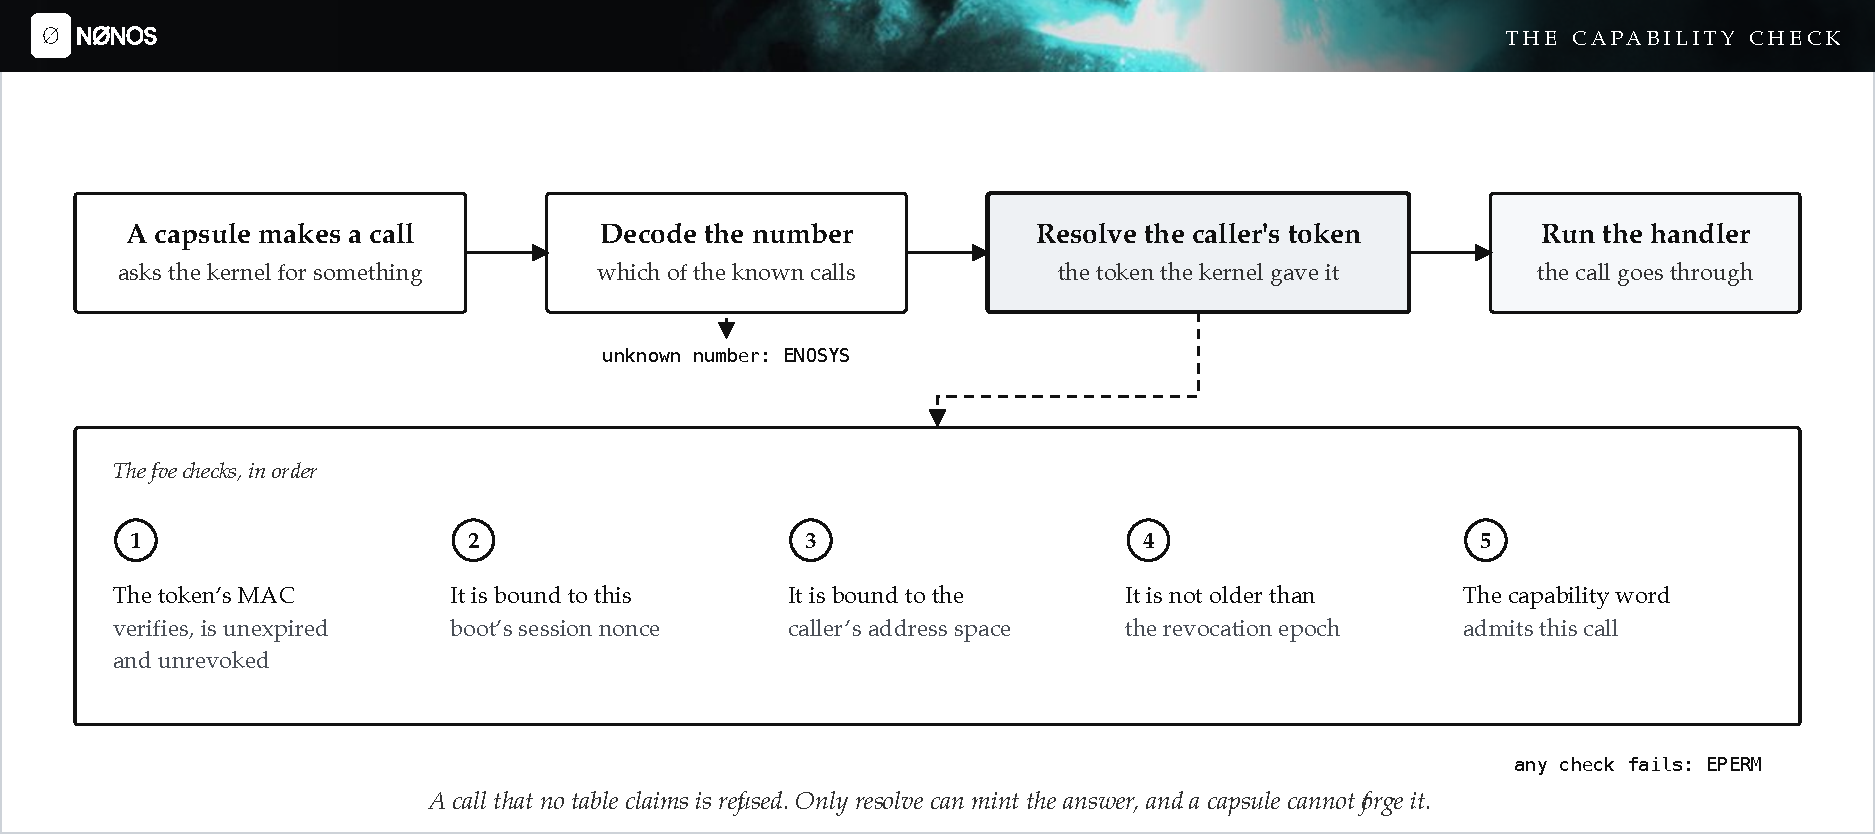
\includegraphics[width=0.84\textwidth]{figures/diagram-capability-check.pdf}
\caption{The capability check on every native system call: decode the number, resolve the caller's token, run five checks in order. Any failure is \code{EPERM}. A number that is not a native call is \code{ENOSYS}, or goes to the guest's supervisor (Section~\ref{sec:box}). Sources: \code{docs/kernel/capabilities-the-check-on.md} and \code{src/syscall/contract/resolver/resolve.rs}.}
\label{fig:capcheck}
\end{figure}

At spawn the kernel installs the word from the verified manifest exactly once. A second call is rejected, so a stale spawn path cannot reissue authority. A request for a bit the manifest does not declare is refused with \code{GrantOutsideManifest}.\srcs{src/process/caps.rs:115-127}{src/security/capsule_manifest/verify/caps.rs:31-39} A new process inherits only a small ambient set from its parent, and an air-gapped boot removes \code{Network} from every capsule.\srcs{src/process/core/table/inherit.rs:52-61}{src/kernel_core/process_spawn/capsule_spawn/runner/profile_gate.rs:48-56}

The documentation is candid about what the word does not do yet. The \code{IO} and \code{Hardware} bits gate nothing. \code{Keyring} and \code{Entropy} gate only kernel clients that no code calls. And the image-wide capability ceiling is computed and logged, not enforced: a capsule that asks for more still starts, and the log prints \code{[CEILING] not enforced, would refuse}.\srcs{docs/kernel/capabilities-what-each-bit.md}{docs/build/profiles.md}

\subsection{IPC}

Each capsule has one inbox, and a service is an endpoint in a registry with the capability bits a sender must hold. A send by name passes four gates: the \code{IPC} bit in the token; the endpoint's required bits; the held-endpoint and peer lists, which restrict who may reach a driver; and a byte budget.\src{docs/kernel/ipc-who-may-send.md} The kernel writes the sender's name itself, so a capsule cannot forge it. A payload is at most 1~MiB; all inboxes together hold at most 96~MiB, one inbox 16~MiB, and one sender at most half an inbox.\src{src/ipc/nonos_inbox/budget.rs:41-43} Reaching any of the 11 services that carry traffic off the machine takes \code{Network} as well as \code{IPC}.\src{src/services/registry/policy.rs:26-38} The peer list still has one entry: the Shield prover may send only to \code{shield.core}.\src{src/services/registry/peers.rs:27-35} Figure~\ref{fig:ipc} shows the gates.

\begin{figure}[t]
\centering
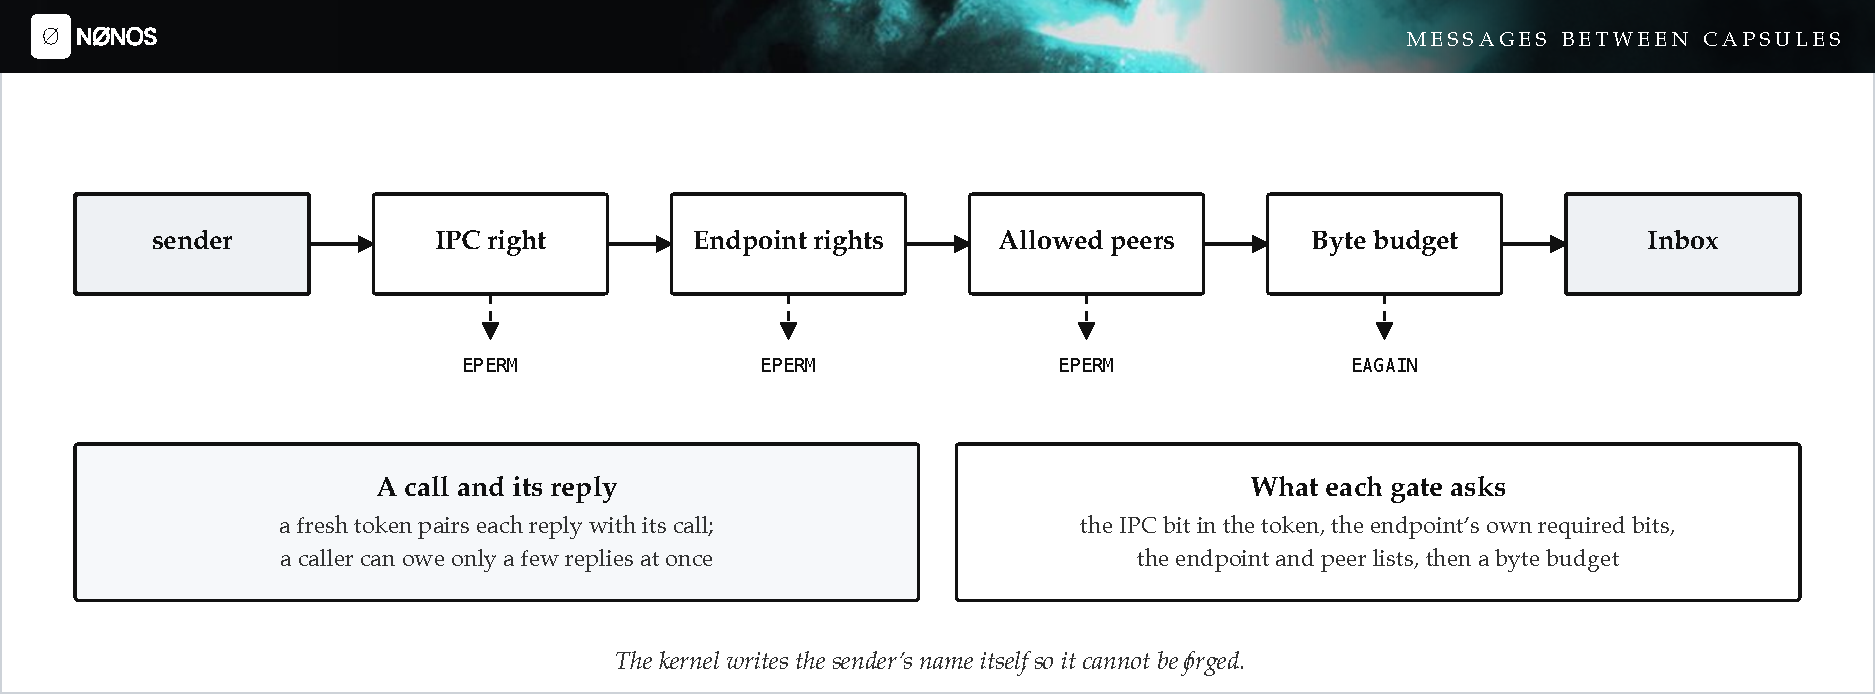
\includegraphics[width=0.84\textwidth]{figures/diagram-ipc-gates.pdf}
\caption{The four gates on a send between capsules, with the error each returns. The kernel stamps the sender's name. Sources: \code{docs/kernel/ipc-who-may-send.md}, \code{src/ipc/nonos\_inbox/budget.rs}.}
\label{fig:ipc}
\end{figure}

\subsection{Drivers and the hardware broker}

A driver capsule claims its device from the broker and then asks for MMIO windows, DMA buffers, interrupt bindings and port I/O, each behind its own capability bit. The broker gives each driver capsule its own IOMMU domain where a unit is in service, and every image turns translation on at boot. Where no unit is in service, a Standard boot goes on with the claim unconfined and says so in four places; Hardened and Air-Gapped stop.\srcs{docs/kernel/iommu-per-capsule-domains.md}{docs/release/0.9.3-security-limits.md} On release the broker stops bus mastering before it frees DMA frames.\src{docs/overview/threat-model-a-hostile-or.md}

\begin{table}[t]
\centering
\caption{The 67 driver capsules by class, generated from the \code{userland/capsule\_driver\_*} directories that hold a \code{Capsule.mk}. Which of them have run on real hardware and which only in their host model is in the hardware notes, and the answer for most is the second.}
\label{tab:drivers}
% generated by paper/tools/gen_tables.py from userland/capsule_driver_*/Capsule.mk
\begin{tabular}{@{}lr>{\raggedright\arraybackslash}p{9.2cm}@{}}
\toprule Class & Count & Drivers\\ \midrule
Storage & 12 & {\footnotesize \texttt{ahci}, \texttt{nvme}, \texttt{piix\_ide}, \texttt{buslogic}, \texttt{mpt}, \texttt{pvscsi}, \texttt{storvsc}, \texttt{ufs}, \texttt{sdhci}, \texttt{rtsx}, \texttt{virtio\_blk}, \texttt{virtio\_scsi}}\\
USB & 17 & {\footnotesize \texttt{xhci}, \texttt{ehci}, \texttt{ohci}, \texttt{uhci}, \texttt{usb\_hub}, \texttt{usb\_hid}, \texttt{usb\_msc}, \texttt{usb\_audio}, \texttt{usb\_mic}, \texttt{uvc}, \texttt{ccid}, \texttt{fido}, \texttt{cdc\_acm}, \texttt{cdc\_ecm}, \texttt{cdc\_ncm}, \texttt{rndis}, \texttt{bt\_usb}}\\
Wired network & 14 & {\footnotesize \texttt{e1000}, \texttt{e1000e}, \texttt{igb}, \texttt{igc}, \texttt{ixgbe}, \texttt{rtl8139}, \texttt{rtl8153}, \texttt{rtl8169}, \texttt{ax88179}, \texttt{pcnet}, \texttt{tulip}, \texttt{virtio\_net}, \texttt{vmxnet3}, \texttt{netvsc}}\\
Wi-Fi & 5 & {\footnotesize \texttt{iwlwifi}, \texttt{mt7921}, \texttt{rtl8821ce}, \texttt{rtl8822ce}, \texttt{rtl8852be}}\\
Input & 5 & {\footnotesize \texttt{ps2\_input}, \texttt{i2c\_hid}, \texttt{spi\_hid}, \texttt{virtio\_input}, \texttt{vmmouse}}\\
Display & 5 & {\footnotesize \texttt{bga}, \texttt{bootfb}, \texttt{intel\_display}, \texttt{virtio\_gpu}, \texttt{vmware\_svga}}\\
Audio & 2 & {\footnotesize \texttt{hda}, \texttt{ac97}}\\
Buses & 4 & {\footnotesize \texttt{gpio}, \texttt{i2c\_pci}, \texttt{spi}, \texttt{smbus}}\\
Virtual machine guests & 3 & {\footnotesize \texttt{virtio\_rng}, \texttt{vmbus}, \texttt{vmmdev}}\\
\midrule Total & 67 & \\
\bottomrule
\end{tabular}

\end{table}

\note{\path{docs/release/0.9.3-supported-hardware.md}; \path{docs/hardware/MATRIX.md}.}The 0.9.2 changelog tree had 18 driver capsules, so 49 arrived between the two trees. Each is a ring-3 process with a claim on its own device. A driver whose device is missing leaves at once, and one whose device fails gives up after a few seconds.\note{\path{README.md}, section "Drivers".} We say clearly what this does not mean. Most of the new drivers have been exercised against a model of the chip or under QEMU. On QEMU the e1000, e1000e, igb, RTL8139, PCnet, vmxnet3 and Tulip drivers each obtained a DHCP lease; the RTL8821CE has one hardware report; the other Wi-Fi drivers have run only against modelled devices.\note{\path{docs/release/0.9.3-what-is-new.md}, section "Drivers"; \path{docs/release/0.9.3-known-issues.md}, section "Hardware".}

\section{The trust chain}\label{sec:chain}

Each stage holds the next to keys and roots compiled into itself, and the kernel also looks back at the loader (Figure~\ref{fig:boot}). This part of the design is unchanged from 0.9.2 in structure. What 0.9.3 adds is boots, with a caution about which ones count. The development images that most of the evidence directories use carry path-only trailers, with no STARK proof, so they exercise the Merkle-path half of the gate and not the proof half. The proof half has run on sealed release images: the release-sealed boot of 26 October has every capsule spawned and attested as \code{vendor}, and the screenshot below is a sealed image under KVM. The 0.9.2 paper could say only that the release was built and held by host tests.\srcs{docs/release-evidence/0.9.3/README.md}{docs/release-evidence/0.9.3/release-sealed-crash/README.md}

\begin{figure}[t]
\centering
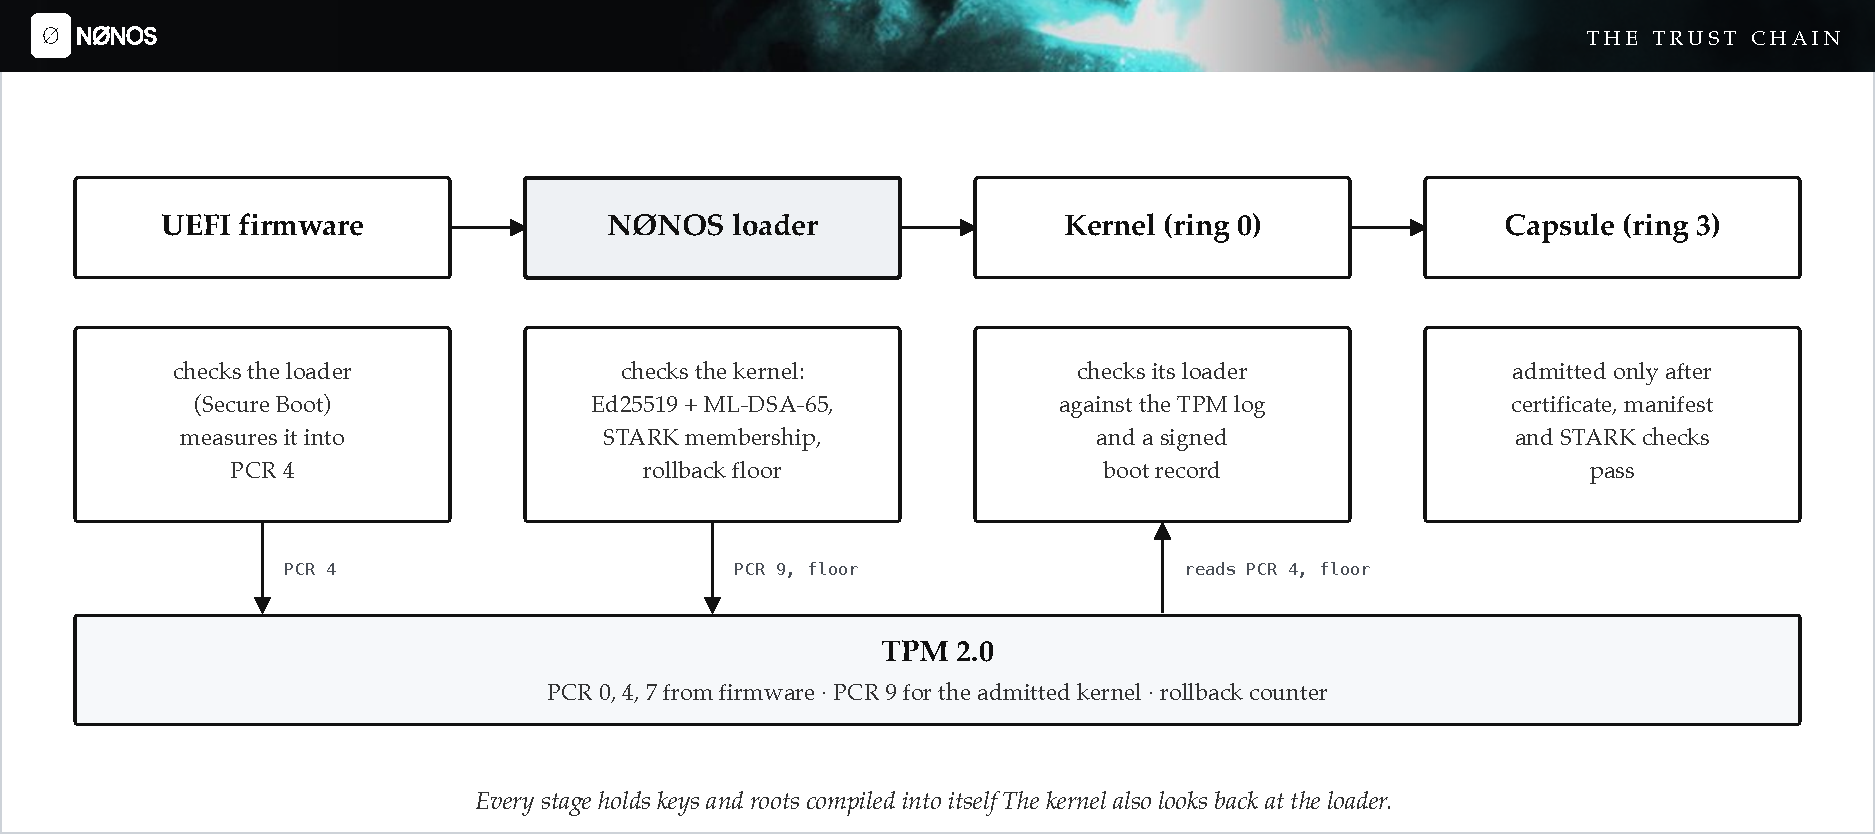
\includegraphics[width=0.84\textwidth]{figures/diagram-boot-chain.pdf}
\caption{The boot chain and the TPM registers each stage uses. Firmware measures the loader into PCR 4; the loader checks the kernel and extends PCR 9; the kernel checks the loader back against the TPM's event log and a signed boot-root record, then checks every capsule. Sources: \code{docs/security/boot-chain-and-signatures.md}, \code{docs/security/measured-boot-and-tpm.md}.}
\label{fig:boot}
\end{figure}

\subsection{The loader checks the kernel}

The kernel image carries a signature blob (\code{NKRSIG2}) with an Ed25519 signature and an ML-DSA-65 signature, each over the same 36-byte message: the BLAKE3 hash of the kernel ELF followed by the rollback index.\src{nonos-bootloader/tools/sign-kernel/src/message.rs:17-22} The public halves are compiled into the loader, and a production loader refuses to build without the ML-DSA-65 key.\src{nonos-bootloader/build.rs:135-216} The loader's pipeline runs the signature and rollback check, then \code{attest\_kernel} for the STARK trailer, then raises the TPM rollback floor, and only then hands over.\src{nonos-bootloader/src/entry/pipeline.rs:30-50} A kernel whose trailer fails is refused in every mode, development included.\src{nonos-bootloader/src/boot/attestation/kernel_gate.rs:34-60}

Figure~\ref{fig:bootshot} is the loader's screen on the sealed 0.9.3 image. It lists the ten steps, and step 7 is "Kernel STARK proof". The screen also says what was not there: Secure Boot off, no TPM, "TPM OFF: no TPM 2.0 measured boot". That run was under KVM, which gives the guest no TPM, so the chain's TPM half did not run in it.

\begin{figure}[t]
\centering
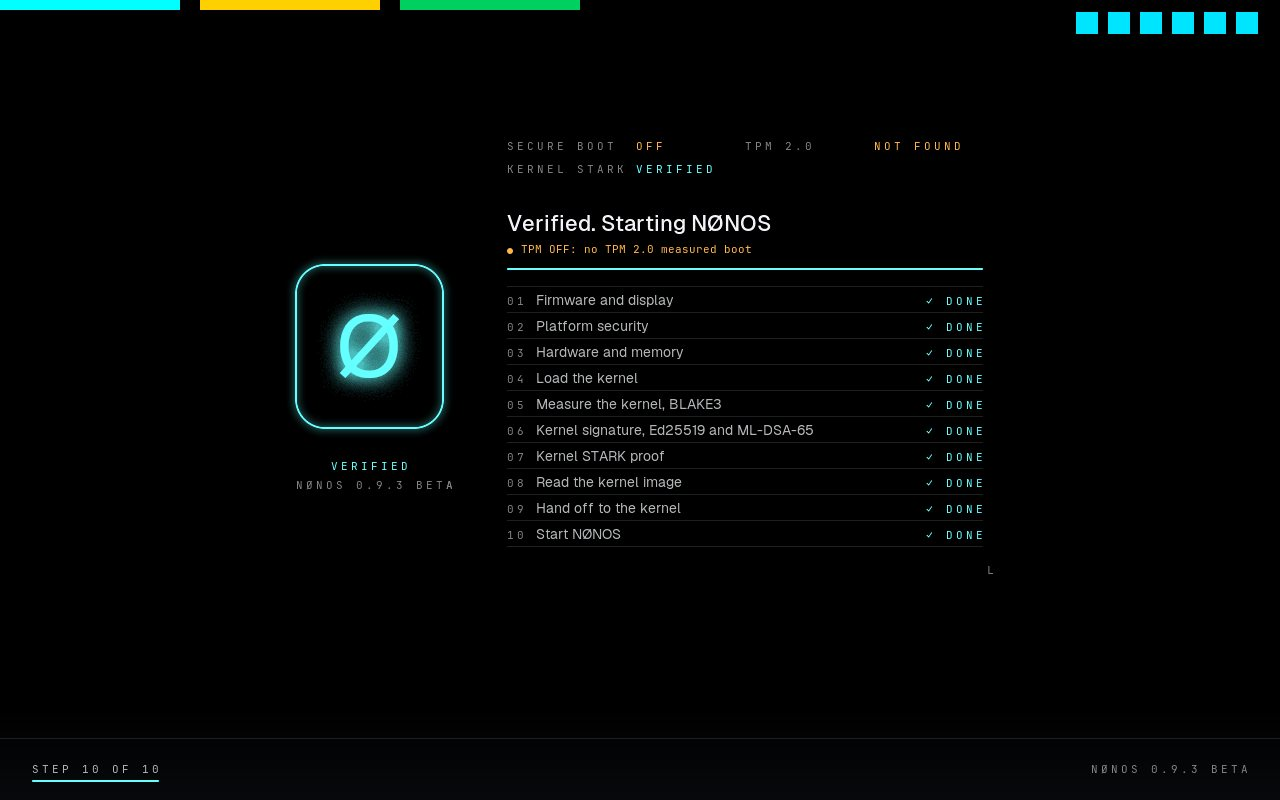
\includegraphics[width=0.55\textwidth]{figures/boot-verified.jpg}
\caption{The loader's screen on the sealed 0.9.3 image, under KVM, with no TPM and Secure Boot off, both shown in orange at the top. Steps 5 to 7 measure the kernel with BLAKE3, check the Ed25519 and ML-DSA-65 signatures, and check the kernel's STARK proof. This is one boot of one image on a virtual machine; it shows the kernel proof checked and says nothing about the TPM path or about a machine with Secure Boot on.}
\label{fig:bootshot}
\end{figure}

\subsection{The kernel checks its loader}

Before init, \code{check\_bootloader} replays the firmware's TCG event log, requires it to reproduce the live PCR~4, takes the last application the log names as the loader, and holds that Authenticode digest to a 104-byte boot-root record signed with an ECDSA P-256 device-policy key compiled into the kernel, and to the loader's own STARK slot.\note{\path{nonos-boot-measure/src/gate/verdict.rs:22-58}; \path{docs/security/boot-chain-and-signatures.md}, section "The kernel checks its loader".} No program starts if the check refuses or finds no evidence.\src{src/kernel_core/init/entry/loader_refusal.rs:27-48} Without a TPM or a log, the kernel falls back to hashing the loader file the loader handed it, and says so in its verdict. That check then rests on the loader's own word.\srcs{nonos-boot-measure/src/gate/verdict.rs:60-75}{src/security/boot/loader_check/run.rs:34-55}

\subsection{The kernel checks every capsule}

A capsule ships its ELF with a \nonos{} ID certificate signed by the trust anchor, a manifest signed by its publisher, and an attestation trailer. \code{preflight} runs \code{verify\_id\_cert}, \code{verify\_with\_publisher} and \code{attest\_gate} in that order. Certificates and manifests need one valid signature of each algorithm. The manifest check covers eight conditions, from the certificate hash to the declared endpoints.\srcs{src/kernel_core/process_spawn/capsule_spawn/runner/preflight.rs:36-76}{src/security/capsule_manifest/verify/mod.rs:37-62} Section~\ref{sec:capsules} goes through admission.

\subsection{The STARK gate and its statement}

Every gate checks one statement: under root $R$, the leaf built from context $C$ with kind $K$ is a slot of a 256-slot tree. The gate builds $C$ itself from what it is about to run and grant. For a capsule, $C$ is 48 bytes: the BLAKE3 hash of the ELF, the capability word (8 bytes) and the policy epoch (8 bytes). For a kernel or loader, $C$ is the measurement and the boot epoch.\src{nonos-attest-path/src/context.rs:23-40} The leaf is a Poseidon permutation over the Goldilocks field of a domain word, the digest of $C$ and the kind, so a capsule slot cannot open as a kernel.\src{nonos-attest-path/src/leaf.rs:51-71}

The gate checks the statement twice, once by folding the Merkle path in the trailer up to the root, and once by running \code{nox\_verify} on a transparent STARK proof of the same slot. It admits only when both pass, and the root is always the gate's own compiled-in or signed value, never the trailer's.\src{src/security/capsule_attest/path.rs:45-53} The proof system is hash-based, with a Fiat-Shamir transcript, no trusted setup and no pairing. A trailer carries at most 256~KiB of proof.\src{nonos-attest-path/src/v4/layout.rs:32}

Three trees exist: the capsule policy tree, checked by the kernel at every spawn; the kernel tree, checked by the loader; and the bootloader tree, whose root is signed into the boot-root record because it cannot live inside the loader it measures.\note{\path{docs/security/stark-attestation.md}, section "Three trees".} \code{nonos-stark-enroll} builds them on the enrolling host, checks every proof with the gates' own verifier before writing it, and records a transcript from which anyone can recompute the root.\src{nonos-stark-enroll/src/stark/prove.rs:28-67} Figure~\ref{fig:who} shows where proofs are made and where they are checked.

\begin{figure}[t]
\centering
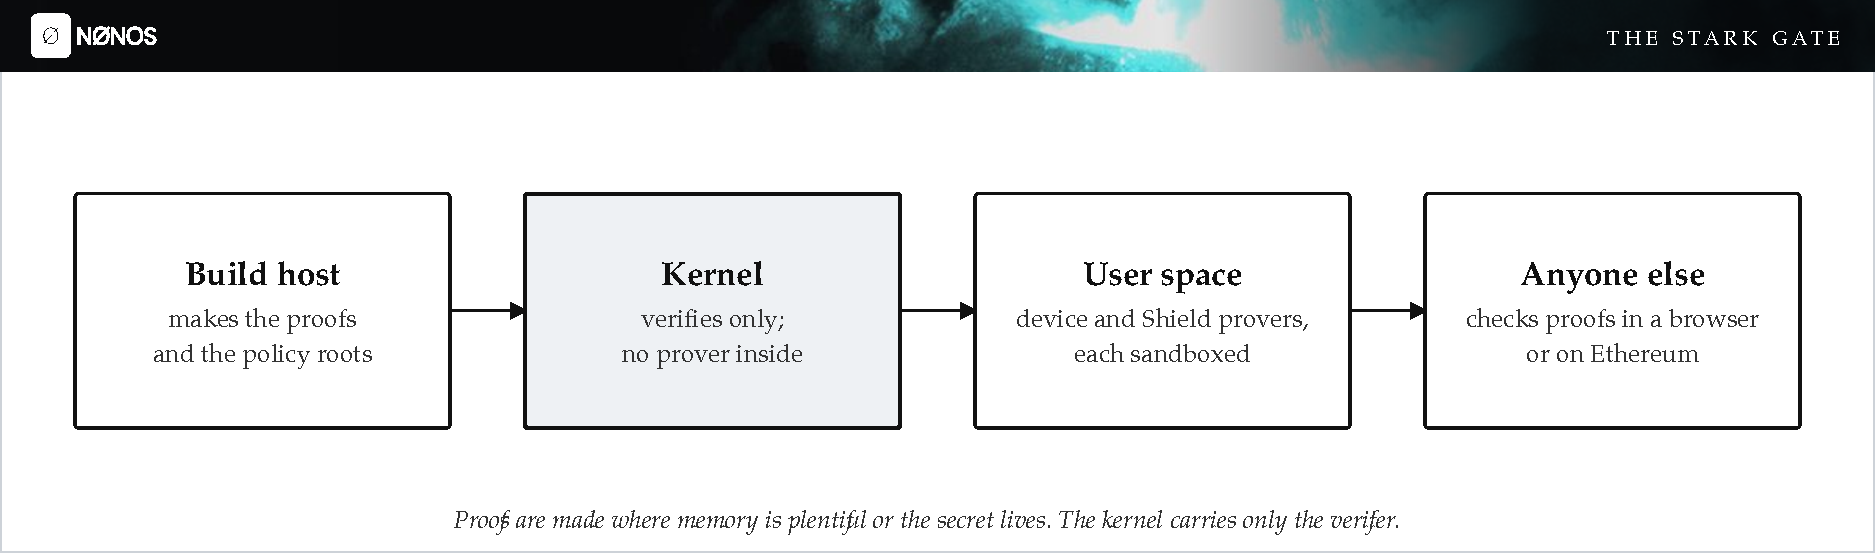
\includegraphics[width=0.84\textwidth]{figures/diagram-who-proves.pdf}
\caption{Who proves and who verifies. Proofs are made where memory is plentiful or where the secret lives. The kernel carries only the verifier. Sources: \code{README.md}, \code{docs/security/stark-attestation.md}.}
\label{fig:who}
\end{figure}

A trailer does not prove that the image is signed, that the capsule's code behaves, which slot it occupies (the path travels in the clear), or freshness by epoch. The path check rests on Poseidon's collision resistance and the proof's soundness on the STARKs repository, and no proof in the tree covers either.\note{\path{docs/security/stark-attestation.md}, section "What a trailer does not prove".} For this paper the middle item matters most. A STARK of membership is an identity statement. It says nothing about what a program does once it runs, and that is why Section~\ref{sec:box} exists.

\subsection{Measured boot, sealed keys and quotes}

The TPM never stores a \nonos{} key. The kernel asks it to derive keys under a PCR policy each time. The machine key, an HMAC under a primary key whose policy is the current value of PCRs 0, 4, 7 and 9, protects the data volume and sealed records, so the same disk in another machine, or the same machine in another boot state, gets another key.\srcs{src/security/tpm/machine_key/derive.rs:32-57}{src/security/tpm/machine_key/pcrs.rs:21-24} The device secret is derived under a policy the release signs over PCR~9, combined with this machine's PCRs 0, 4 and 7, so an approved kernel update keeps it while a firmware or loader change does not.\src{src/security/tpm/device_secret/derive.rs:33-54}

Two things are new in 0.9.3. A data volume formatted on a boot the release approved now has a random key, wrapped under a key the TPM gives only to a kernel the release approved. And an installed disk can be updated in place: from the moment the installed system prepares an update until the next boot, a one-boot handover record carries the key across a new bootloader. On QEMU with a software TPM, a prepared volume opened under an image with a changed bootloader through the handover, and then under that bootloader's own key. The window in which the handover record exists is a known weakness, listed in Section~\ref{sec:limits}.\note{\path{docs/release/0.9.3-what-is-new.md}, section "Update NØNOS (keep my data)"; \path{docs/release-evidence/0.9.3/s1-k1-update/README.md}.}

\code{MkAttestDoc} answers a 32-byte challenge with a TPM quote over PCRs 0, 1, 2 and 7. Because the attestation key is the same on every boot, a quote names the machine, so the kernel releases it only to a capsule that holds \code{AttestRead} and does not hold \code{Network}.\src{src/syscall/caps/checks/system.rs:40-52} The quote covers firmware state and not the PCRs \nonos{} itself extends; a design to quote the \nonos{} chain exists and is marked as design, with nothing landing before the 0.9.3 seal.\src{docs/design/k1-attest-doc-v4.md}

\subsection{The anonymous device proof}

\code{nonos-device-attest} proves, to a verifier who learns nothing else, four facts together: an approved bootloader started the machine, an approved kernel runs on it, the machine is an enrolled device, and a tag is this device's tag for the verifier's scope. The proof is made on the booted machine in a capsule that has no network bit and is the only one allowed \code{DeviceSecret}.\srcs{nonos-device-attest/README.md}{userland/capsule_prove/Capsule.mk:17-35} Its own README lists it as built and never run on a booted image, and we do not claim otherwise.\note{\path{nonos-device-attest/README.md}, section "What is not done".}

\section{Capsules}\label{sec:capsules}

\subsection{What a capsule is}

A capsule is a statically linked position-independent ELF built offline for the target \code{x86\_64-nonos-user}, plus three files: a \nonos{} ID certificate, a binary manifest and an attestation trailer. Authors do not write manifests. They set \code{CAPSULE\_*} variables in a \code{Capsule.mk}, and the build produces the manifest.\srcs{docs/userland/README.md}{docs/userland/manifests-and-capabilities.md} There are 152 \code{Capsule.mk} files in the tree. Each names the capsule's service, its endpoints and its capability word, and the same facts appear again in the kernel's own copy, which a script holds to the manifest.\src{scripts/check_mirror_caps.py}

\subsection{The manifest}

The manifest is schema version 3 and big-endian. In wire order it carries the schema version; a certificate id, the BLAKE3 hash of the \nonos{} ID certificate; a namespace of 1 to 96 bytes; a version; the target triple; a payload hash, the BLAKE3 hash of the whole ELF; the required capability word; the optional word, which must not overlap the required one; up to 16 endpoints; and one to four signatures.\srcs{src/security/capsule_manifest/schema/constants.rs:17-25}{src/security/capsule_manifest/decode/mod.rs:25-47} The publisher signs every byte before the signature count. Algorithm 1 is Ed25519 with 64-byte signatures and algorithm 3 is ML-DSA-65 with 3309-byte signatures.\src{src/crypto/asymmetric/alg_id/lengths.rs:19-26}

\subsection{Admission}

Figure~\ref{fig:admit} shows admission at spawn. The certificate must verify under the trust anchor with both algorithms, must not be stale or revoked, and bounds what the publisher may request through a capability ceiling and namespace globs. The manifest must then verify under the publisher's keys with both algorithms, and its payload hash must equal the BLAKE3 of the ELF being loaded. Finally the STARK gate checks the capsule's slot under the compiled-in policy root, with the manifest's required capability word as part of the statement. A capsule enrolled with one set of rights therefore cannot open with another.\src{src/kernel_core/process_spawn/capsule_spawn/runner/preflight.rs:36-76} Only after all three checks does the kernel create the process, install the word and record the measurement in the attestation registry.

\begin{figure}[t]
\centering
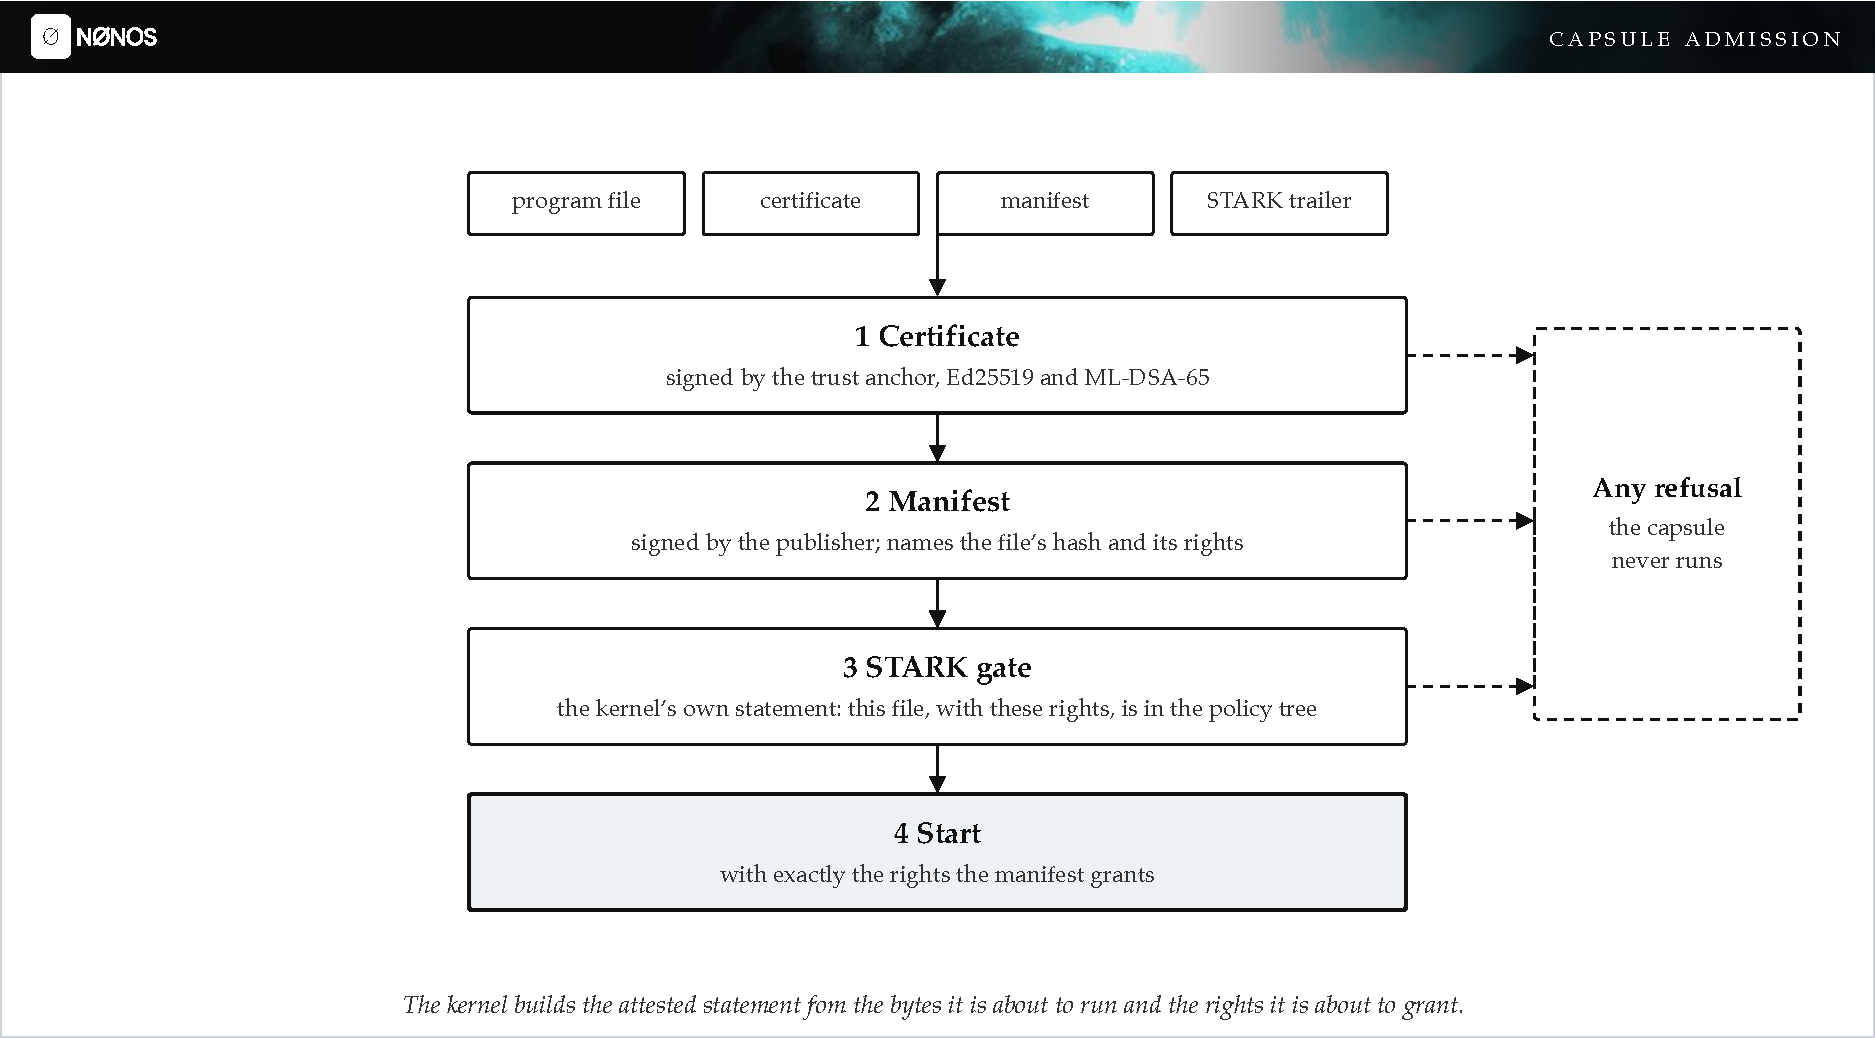
\includegraphics[width=0.84\textwidth]{figures/diagram-capsule-admission.pdf}
\caption{Capsule admission. The kernel builds the attested statement from the bytes it is about to run and the rights it is about to grant. Any refusal means the capsule never runs. Sources: \code{docs/security/boot-chain-and-signatures.md}, \code{docs/security/stark-attestation.md}.}
\label{fig:admit}
\end{figure}

A second admission path exists for code built on the machine itself. When the vendor root refuses a capsule, the kernel tries roots the person enrolled locally, and under such a root a trailer is a keyed tag the kernel minted for a local build instead of a STARK proof. The serial line \code{[ZK-ATTEST] ok} names the authority that admitted each capsule.\srcs{src/security/capsule_attest/against_root.rs:31-45}{docs/security/stark-attestation.md} The publisher tier, under which a capsule outside the project's namespace could run on its publisher's signature, admits no capsule in the release image.\src{docs/userland/signing-and-publisher-keys.md}

\subsection{An example: the Linux personality}

The capsule that matters most for this release is \code{capsule\_linux}, the Linux personality. Its \code{Capsule.mk} requires the word \code{0x104001979}: \code{CoreExec}, \code{IPC}, \code{Memory}, \code{Crypto}, \code{FileSystem}, \code{Debug}, two graphics bits, \code{StoreWrite} and \code{ForeignExec}. It lists \code{Network}, \code{LocalSign} and \code{StreamImport} as optional, with the word \code{0x600000004}.\src{userland/capsule_linux/Capsule.mk:50-59} The kernel holds a copy of the same list, and a comment there says the manifest is what the gate enforces.\src{src/userspace/capsule_linux/spawn.rs:36-55}

Two things about that word are worth stating, because Section~\ref{sec:box} depends on them. \code{ForeignExec} is the right to create a process the kernel has not verified, build its address space and answer its calls, and \code{capsule\_linux} is the only capsule in the tree whose \code{Capsule.mk} requests it.\src{docs/security/capsule-isolation-the-linux-personalitys.md} And \code{Network} is optional: it is held only by the instances that need it, which the personality's roles decide when they start, not by the program inside.\src{src/userspace/capsule_linux/roles.rs:32-58}

\subsection{Other capsules relevant to keys}

The keyring capsule holds the wallet's keys with no file, network or device access. It generates 12-word BIP-39 phrases, derives keys on \code{m/44'/60'/0'/0/i} for up to 8 accounts, and signs EIP-1559 transactions with in-process secp256k1, and it seals or opens the wallet's records only for a sender the service registry names as the wallet.\srcs{userland/capsule_keyring/src/server/hd.rs:37-60}{userland/capsule_keyring/src/server/vault_gate/mod.rs:17-25} The one caveat that matters is old: any capsule that holds both \code{Crypto} and \code{FileSystem} can ask the kernel for the vault root under its published label and read the sealed blob under \code{/data}, and the Linux personality, Settings and the Terminal are among those that hold both.\src{docs/security/protections-and-limits-what-nonos-does.md}

\section{Running other people's programs}\label{sec:box}

This section is the argument of the release. It has three parts: why a daily machine must run programs it cannot vouch for, how a capability microkernel turns a short signed list into enforcement, and what we saw when we tried to get past it.

\subsection{Why the machine has to}

The case for refusing everything we did not sign is easy to make and hard to live with. A machine that runs only the project's own capsules can be proved, in the sense of Section~\ref{sec:chain}, down to the byte. It also has no password manager the person has used for years, no Telegram, no \code{git}, no Monero command-line wallet and no way to open a PDF that arrived by email. People route around a machine like that. They keep the real work on another computer, which is the computer the proofs were meant to protect them from.

So the machine has to run programs written by others, and the ones people want are not small. KeePassXC 2.7.8 is a Qt~5 application. Telegram Desktop 5.0.1 is Qt~6 with 254 packages in its install. Neither will be rewritten as a capsule. The honest options are to run them as they are, or not to run them.

Running them as they are raises a second question that most systems answer badly: what does the program get? On a typical desktop, a program started by the person has the person's authority. It can read their files, signal their other programs, open any socket and start any tool. The permission model, where there is one, is a set of dialogs answered by someone who cannot see what is behind them. A Linux password manager that wants the network and a Linux image viewer that wants the network are indistinguishable at the prompt.

\nonos{} makes a different trade. A program gets a box, the box is a short list fixed in advance and signed with the program's Marketplace listing, and anything not on the list is refused with a message that says why. The person decides before install, by reading the list, not at runtime, by guessing.

\subsection{Why a capability microkernel fits}

Holding a program to a list is an old idea, and the usual trouble is where the check lives. In a monolithic kernel the check is a patchwork of hooks on the paths a program might take, and a missed path is a hole. A capability microkernel starts from the other side. A process has nothing unless it holds a capability, and almost every service a program could want is a message to a named capsule that has its own capability word.

That structure gives the box three properties, and they are the reason the design is built the way it is.

First, the guest holds nothing. A Linux program is a process created with an empty capability word. The kernel installs the word with \code{install\_spawn(pid, 0)} and logs \code{[FOREIGN] guest pid=... caps=...} with the mask read back, so the log states what the guest holds instead of assuming it.\src{src/process/foreign/spawn_guest.rs:41-48} With no bits, every native call a guest could make fails the cap table. The one exception is \code{MkTtyQuery}, which only describes the caller's own streams.\src{src/syscall/contract/cap_table/mk_surface.rs:56-60} A guest that learns \nonos{}'s system-call numbers gains nothing, because it has no token that admits them.

Second, every other call goes to one place. A Linux system call number is a small integer, and \nonos{} native numbers are four ASCII letters, so the kernel does not recognise a Linux call. It parks the guest thread and wakes the capsule that created it, its supervisor.\src{src/process/foreign/trap.rs:28-57} The supervisor is \code{capsule\_linux}, the personality. It is the only capsule that holds \code{ForeignExec}, and the kernel lets it touch only the guests it made: the peer calls that map, copy, protect and unmap guest memory begin with \code{supervised\_asid}, which refuses any pid the caller does not supervise.\srcs{src/process/foreign/peer_guard.rs:64-73}{docs/security/capsule-isolation-the-linux-personalitys.md} One supervisor holds at most 1,024 guests and threads.\src{src/process/foreign/room.rs:33-37} So there is no path from a guest to the world that does not pass through the personality, and the kernel, not the personality, guarantees it.

Third, the checker is itself a capsule. It is signed, enrolled under the policy root and admitted by the STARK gate like any other, and it holds a fixed capability word. If the checker has a bug, the damage is bounded by that word, which Section~\ref{sec:capsules} listed. This is weaker than it sounds and stronger than the alternative. It is weaker because the word includes \code{FileSystem} and \code{Crypto}. It is stronger because the checker is a small ring-3 program with a published word, not a patchwork inside the kernel.

Figure~\ref{fig:box} draws the path of one call.

\begin{figure}[t]
\centering
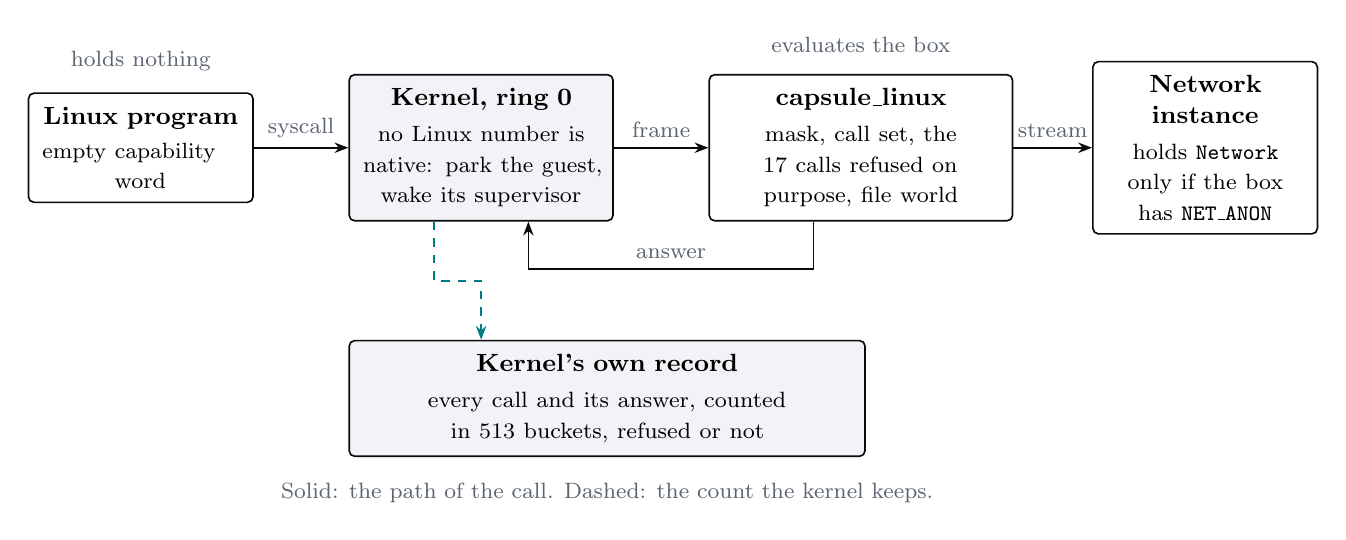
\begin{tikzpicture}[
  font=\small,
  box/.style={draw=ink,line width=0.6pt,rounded corners=2pt,align=center,inner sep=5pt,minimum height=1.35cm,fill=white},
  ring0/.style={box,fill=paper},
  note/.style={font=\footnotesize,text=mute,align=center},
  arr/.style={-{Stealth[length=5pt]},line width=0.6pt,draw=ink},
  darr/.style={-{Stealth[length=5pt]},line width=0.6pt,draw=teal,dashed}]
\node[box,text width=2.5cm] (g) {\textbf{Linux program}\\[2pt]\footnotesize \hbox{empty capability} word};
\node[ring0,text width=3.0cm,right=1.2cm of g] (k) {\textbf{Kernel, ring 0}\\[2pt]\footnotesize no Linux number is native: park the guest, wake its supervisor};
\node[box,text width=3.5cm,right=1.2cm of k] (p) {\textbf{capsule\_linux}\\[2pt]\footnotesize mask, call set, the 17 calls refused on purpose, file world};
\node[box,text width=2.5cm,right=1.0cm of p] (n) {\textbf{Network instance}\\[2pt]\footnotesize holds \code{Network} only if the box has \code{NET\_ANON}};
\draw[arr] (g) -- node[above,note]{syscall} (k);
\draw[arr] (k) -- node[above,note]{frame} (p);
\draw[arr] (p) -- node[above,note]{stream} (n);
\draw[arr] ([xshift=-0.6cm]p.south) -- ++(0,-0.6) -| node[pos=0.25,above,note]{answer} ([xshift=0.6cm]k.south);
\node[ring0,text width=6.2cm,below=1.5cm of k,xshift=1.6cm] (h) {\textbf{Kernel's own record}\\[2pt]\footnotesize every call and its answer, counted in 513 buckets, refused or not};
\draw[darr] ([xshift=-0.6cm]k.south) -- ++(0,-0.75) -| ([xshift=-1.6cm]h.north);
\node[note,above=0.15cm of p] {evaluates the box};
\node[note,above=0.15cm of g] {holds nothing};
\node[note,below=0.2cm of h] {Solid: the path of the call. Dashed: the count the kernel keeps.};
\end{tikzpicture}

\caption{What happens to one Linux system call from a program in a box. The kernel parks the call and hands it to the one supervisor; the supervisor checks the call against the program's policy; the kernel counts the call and the answer in its own record. The program's native capability word is empty. Sources: \code{src/process/foreign/trap.rs}, \code{userland/capsule\_linux/src/linux/app/}, \code{src/process/foreign/seal/}.}
\label{fig:box}
\end{figure}

A word about what we do not say. It is tempting to write that the kernel checks the box on every call. The code says something more careful. The kernel guarantees that every call reaches the checker and that a guest has no other way out. The box itself, the mask and the declared call set, is evaluated by \code{capsule\_linux}. The kernel also keeps a record of its own: it counts every call and its answer into 513 buckets, split into refused and not refused, as the answer is posted, so the record and the answer cannot part.\srcs{src/process/foreign/seal/hist.rs:16-49}{src/process/foreign/seal/absorb.rs:30-38} The two work together. The personality refuses a call outside the declared set with \code{EPERM}, which lands on the refused side of the kernel's count, so a record of a run can show that the box held without trusting what the personality says about itself.\src{userland/capsule_linux/src/linux/app/calls.rs:16-56} Whether that record is checked end to end on a booted release is a separate question, and Section~\ref{sec:box-limits} answers it.

\begin{figure}[t]
\centering
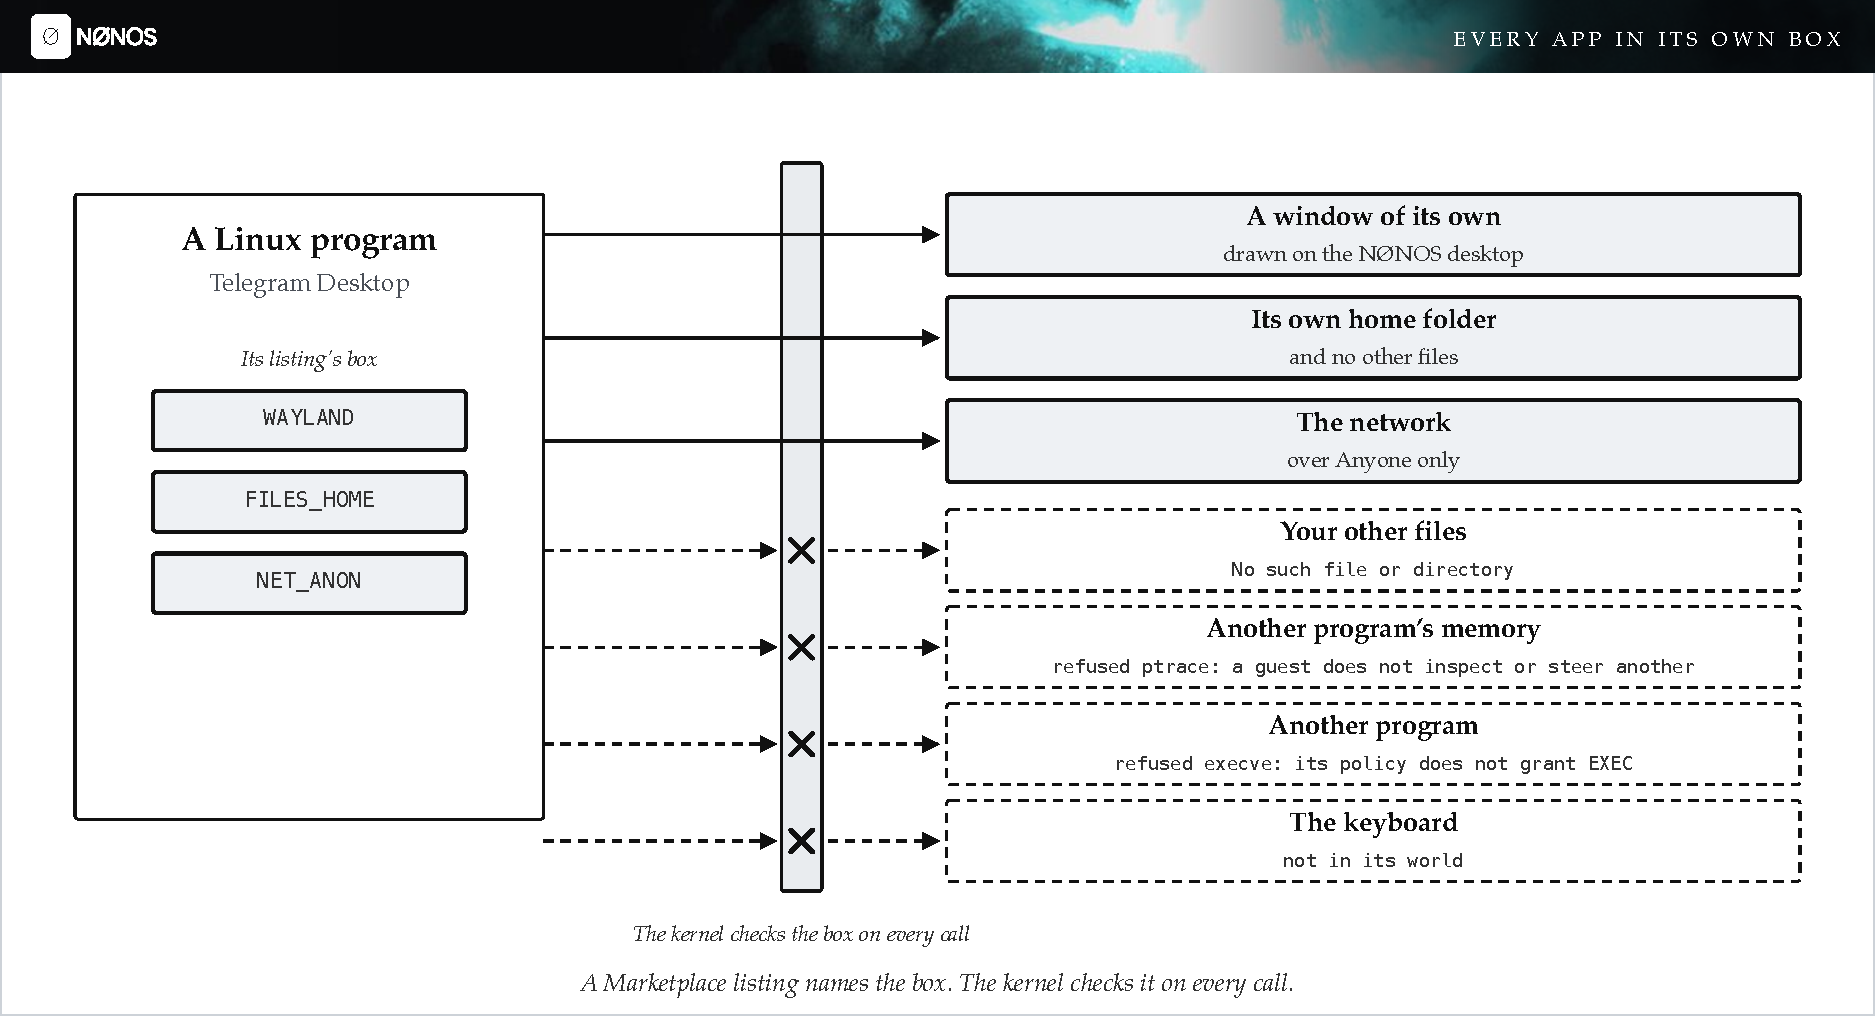
\includegraphics[width=0.84\textwidth]{figures/diagram-the-box.pdf}
\caption{What a program in a box reaches, drawn for Telegram Desktop, whose listing grants \code{WAYLAND}, \code{FILES\_HOME} and \code{NET\_ANON}. Solid arrows are granted, dashed ones are refused, with the answer shown. The band's phrase, "the kernel checks the box on every call", is the project's; the text above and Figure~\ref{fig:box} say how the checking is divided between the kernel and the personality. \code{NET\_ANON} reaches the network the person chose, over Nym or Anyone, never Direct. Sources: \code{docs/using/linux-box.md}, \code{docs/using/marketplace.md}.}
\label{fig:thebox}
\end{figure}

\subsection{What a box is}

A box is 256 bytes. The layout is fixed: the magic \code{NLXPOL01}, a version, the BLAKE3 of the program, a mask of ten service bits, the listing and release ids, a hash of the destination list, and a bit for each of 512 Linux system-call numbers with one more for the native bucket. The decoder accepts exactly the bytes the encoder writes and refuses a wrong length, a non-zero reserved byte, a mask bit with no meaning, or a call bit past bucket 512, so a policy has one encoding and so one hash.\srcs{userland/nonos_linux_policy/src/layout.rs:16-38}{userland/nonos_linux_policy/README.md:1-20} That hash is what a release signs. The \emph{app id}, a BLAKE3 over the program's hash and the policy's hash, is what the personality notes in the kernel's record, so a proof names the program and its box together and neither can be swapped under the other.\src{userland/nonos_linux_policy/src/identity.rs:16-40}

The ten mask bits are the whole vocabulary. Table~\ref{tab:bits} gives them with the number of the 31 catalogue programs that hold each.

\begin{table}[t]
\centering
\caption{The words a box is written in, and how many of the \nPrograms{} Marketplace programs hold each. Three further words exist in the code: \code{FILES\_USER} (the person's own files), \code{MODELS\_RO} (reading the local models) and \code{SERVE\_ONE} (one listener at a port a policy names); the catalogue generator refuses a recipe that asks for \code{FILES\_USER}, so no listed program has it. Counted from \code{userland/capsule\_market/linux-catalogue.json}; definitions in \code{userland/nonos\_linux\_policy/src/mask.rs}.}
\label{tab:bits}
% generated by paper/tools/gen_tables.py from linux-catalogue.json
\begin{tabular}{@{}llr@{}}
\toprule Box word & What it lets the program have & Programs\\ \midrule
\texttt{WAYLAND} & a window of its own on the desktop & 7\\
\texttt{TTY} & the Terminal & 24\\
\texttt{FILES\_HOME} & its own home folder, and no other files & 31\\
\texttt{EXEC} & starting other programs, each held to the same box & 8\\
\texttt{NET\_ANON} & outbound streams, over Nym or Anyone only & 8\\
\texttt{NET\_LISTEN\_LO} & listening on the machine's own loopback & 3\\
\texttt{JIT} & making code as it runs & 1\\
\bottomrule
\end{tabular}

\end{table}

\begin{description}[leftmargin=0pt,style=unboxed,font=\normalfont\code,itemsep=0.3em]
\item[WAYLAND] A window of its own on the desktop, and the input routed to it. Without it, a program that opens the display socket gets \code{EACCES} and the personality logs \code{refused the display: its policy does not grant WAYLAND}.\src{userland/capsule_linux/src/linux/unix/sock.rs:35-37}
\item[FILES\_HOME] Its own home folder. A guest's \code{/} is a tree in the file store, not the person's file system; \code{/home} and \code{/root} are private to the run and kept in memory; without the word they are the shared tree's, read and never written.\note{\path{userland/capsule_linux/src/linux/file/private/rule.rs:16-40}; \path{docs/userland/linux-personality.md}, section "The filesystem a guest sees".}
\item[NET\_ANON] Outbound streams, through the library that applies the person's chosen route, over Nym or Anyone and never Direct, even when Direct is the default network.\srcs{userland/nonos_linux_policy/src/mask.rs:22-26}{userland/capsule_linux/src/linux/net/guest_route.rs:59-75}
\item[EXEC] Starting other programs. Each program started is held to no more than the program that started it, so a chain of \code{execve} cannot widen the box.\src{userland/nonos_linux_policy/src/mask.rs:63-70}
\item[TTY, NET\_LISTEN\_LO, JIT] The terminal; listening on loopback inside the program's own family; making code as it runs.
\end{description}

A program that arrives with no policy at all gets a default box: the terminal, its own home and \code{EXEC}, every call allowed, no window and no network.\src{userland/nonos_linux_policy/src/unlisted.rs:16-40} The comment in the code calls this a project decision, and says that changing it is changing one constant. It is generous on purpose, so command-line tools keep working. It is also the box on the screenshot in Figure~\ref{fig:refusals}, because the programs run there were typed at the Terminal and have no listing.

\subsection{From a listing to a running program}

A listing is where the box is written down. A Marketplace listing for a Linux program carries the Alpine package, a pin of the package's BLAKE3, the program's licence, and a \code{guest\_policy}: the 256 bytes above, written for the exact program the installer will record. The listing's release is signed by its publisher and the index by the Marketplace operator. A schema-3 Linux release with no policy answers \emph{Missing} and can never be installed.\srcs{docs/userland/marketplace-catalogue.md}{userland/capsule_linux/src/linux/install/market/run.rs:34-62}

An install goes through the six gates in Table~\ref{tab:gates}, then fetches the package and what it needs one package at a time over the chosen route, checks each against the Alpine index the catalogue pins, and records the program whose bytes the policy names. A policy the market does not vouch for refuses the install. A failure names the package and the check that stopped it, for example \code{libzmq-4.3.5-r2 (its checksum did not match the signed index)}.\note{\path{docs/using/marketplace.md}, section "How a listing is checked before it installs"; \path{docs/release/0.9.3-what-is-new.md}, section "Installing Linux apps".}

\begin{table}[t]
\centering
\caption{The six gates a Marketplace release must pass before an install is queued. The window decides nothing on its own: it queues a request, and the kernel asks the market for its verdict again. Source: \code{docs/using/marketplace.md}.}
\label{tab:gates}
\begin{tabular}{@{}l>{\raggedright\arraybackslash}p{10.6cm}@{}}
\toprule Gate & Passes when\\ \midrule
index signature & the operator's signature over the catalogue verifies\\
package present & the release names a package URL, a package hash and a manifest hash\\
publisher signature & the release's publisher signature verifies\\
operator validation & the operator marked the release validated\\
architecture & the release runs on \code{x86\_64-nonos} or \code{x86\_64-linux} and needs kernel ABI 1 at most\\
attestation & the release carries a proof trailer hash, or it is a \code{linux.} listing, whose proof this machine makes after it has checked the bytes\\ \bottomrule
\end{tabular}
\end{table}

\begin{figure}[t]
\centering
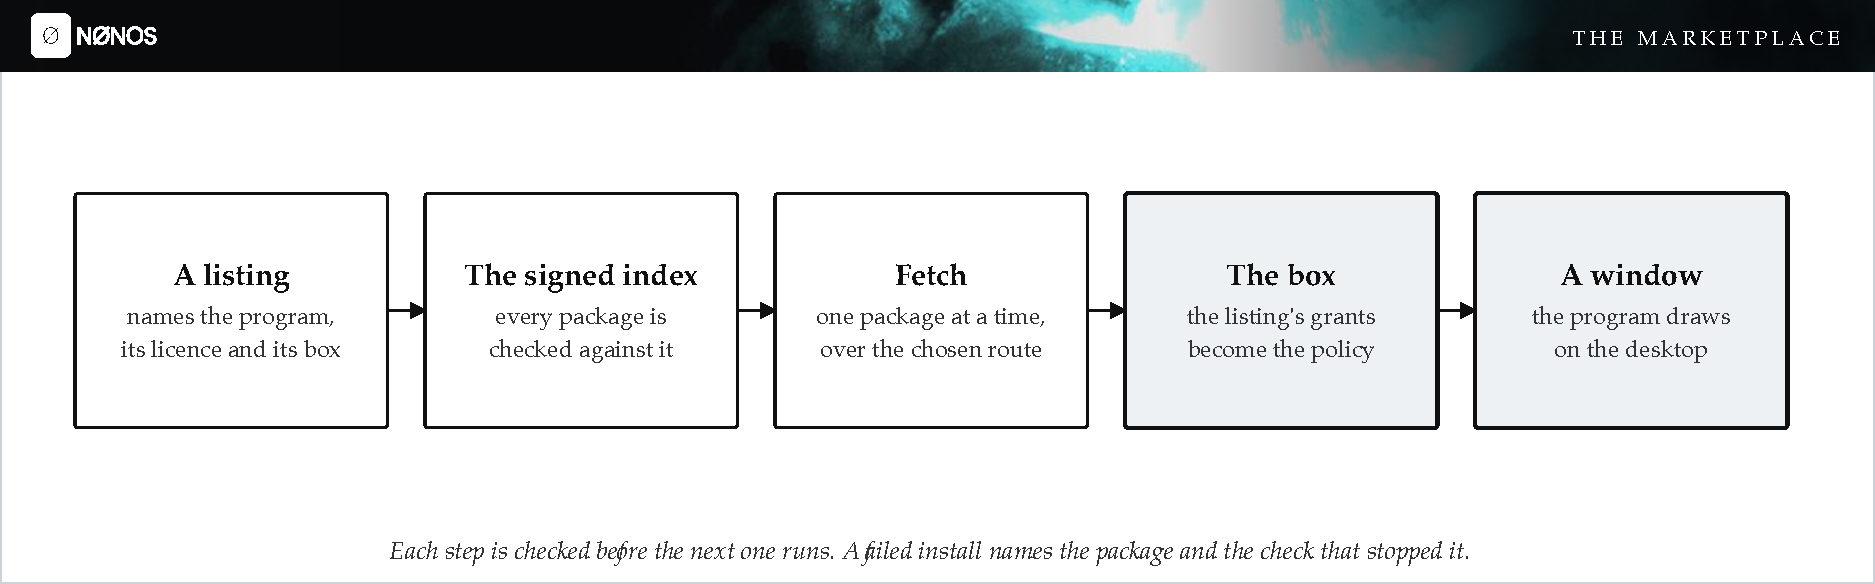
\includegraphics[width=0.84\textwidth]{figures/diagram-install-and-run.pdf}
\caption{From a listing to a window. A listing names the program, its licence and its box; the package is checked against the signed index; the install fetches one package at a time over the chosen route; the listing's grants become the policy; the program draws a window. A failed install names the package and the check that stopped it. Sources: \code{docs/userland/marketplace-catalogue.md}, \code{docs/using/marketplace.md}.}
\label{fig:install}
\end{figure}

The weakest word in that account is "proof". The attestation gate for a Linux listing says that the machine makes the proof itself after checking the bytes. That is the local-authority path of Section~\ref{sec:capsules}, a keyed tag, not a vendor STARK. What the person gets is a chain of checks on identity: the Alpine index signature, the catalogue's pin, the operator's and publisher's signatures, the bytes. The STARK stays with the project's own capsules.\note{\path{docs/using/marketplace.md}, section "How a listing is checked before it installs".} We want the distinction to be plain, because it is the one a reader is most likely to blur. The proof is about \nonos{}'s capsules, and the box is about everyone else's programs.

\subsection{Enforcement, one layer at a time}

The box is enforced in three places, and each does a different job.

\textbf{The kernel's part} is the structure above: an empty word for the guest, one supervisor, peer access only to a supervisor's own guests, a count of every call. It does not know what a Linux call means. The record is explicit that it counts numbers only.

\textbf{The personality's part} is the box itself, and it is done call by call. Before a call is served, a bucket the policy leaves clear is \code{EPERM}, except \code{exit} and \code{exit\_group}, which are served whatever the set says.\srcs{userland/capsule_linux/src/linux/app/rules.rs:21-31}{userland/capsule_linux/src/linux/app/calls.rs:36-56} Beyond that, the personality holds a short list of calls it refuses on purpose with a stated reason: seventeen of them, among them \code{ptrace}, \code{process\_vm\_readv}, \code{process\_vm\_writev}, \code{mount}, \code{chroot}, \code{unshare}, \code{setns} and \code{io\_uring}, which is refused as "a second call path around the gate".\src{userland/capsule_linux/src/linux/serve/refused.rs:21-47} A guest sees only its own processes in \code{/proc}, has no input devices, and cannot name the person's files because they are not in its world.\srcs{docs/release-evidence/0.9.3/s1-isolation-61ec29ea2/README.md}{README.md} An internet socket needs one of \code{NET\_ANON}, \code{NET\_LISTEN\_LO} or \code{SERVE\_ONE}; \code{execve} needs \code{EXEC}.\srcs{userland/capsule_linux/src/linux/net/socket.rs:30-47}{userland/capsule_linux/src/linux/call/spawn/exec.rs:28-31}

\textbf{The network is enforced twice.} The personality never holds \code{Network} in its ordinary run and terminal roles. A program whose box includes \code{NET\_ANON} is started again in a different instance of the personality, \code{app.linux.run.net} or \code{app.linux.term.net}, which does hold the \code{Network} bit, and which exits unless the policy it binds grants \code{NET\_ANON}. A box without \code{NET\_ANON} never runs there; the network role refuses it.\srcs{src/userspace/capsule_linux/run_net.rs:16-34}{src/userspace/capsule_linux/role_term_net.rs:22-44}\src{userland/capsule_linux/src/linux/app/rules.rs:42-61} So for a program without the network word there are two independent refusals: the personality will not make an internet socket, and the instance serving it holds no capability with which the kernel would carry one. That second refusal is the kernel's, and it does not depend on the personality being right.

\subsection{Windows}

The new part of 0.9.3 that a person sees is that a Linux program opens its own window on the \nonos{} desktop. The personality serves a Wayland display to a guest whose box grants \code{WAYLAND}. The guest speaks the Wayland wire protocol over a Unix socket the personality implements: registry, \code{wl\_shm} buffers, \code{xdg} toplevels, seats and keymaps, data devices, output, decoration. The window is registered as a surface with the compositor through the two graphics bits the personality holds, and drawn inside the toolkit's own frame, with a \nonos{} title bar and close, minimise and maximise buttons.\srcs{userland/capsule_linux/src/linux/wayland/mod.rs:19-60}{docs/release-evidence/0.9.3/gui-frame/README.md} A surface's frame callbacks are answered at most 30 times a second, and at once for an idle window.\src{userland/capsule_linux/src/linux/wayland/pace_rule.rs:17-28}

The window is the cheapest thing in the box to give and the most delicate. A guest that holds \code{WAYLAND} can draw anything inside its own window and receive input routed to it. Whether one Linux window can reach another program's surface is a question we have not tested, and it is on the list of things we have not attacked.

What has been shown to run is narrower than the catalogue. On development images, swayimg drew its window, zoomed and closed; its frame's close button ended it with status 0; foot drew its window and ran a shell over \code{/dev/pts}; KeePassXC 2.7.8 drew its welcome screen in a box of \code{WAYLAND} and \code{FILES\_HOME}, once the personality served \code{FUTEX\_WAKE\_OP}, which Qt~5 uses to wake a waiting thread. On a KVM run of the release tree, Telegram Desktop installed from the real Alpine mirror over Anyone and drew its welcome screen. No sign-in or sent message was shown. mpv and zathura are listed and no boot in the evidence shows a window for either. DarkFi's chat app is listed and no boot shows its window. Mousepad is not listed, because on the release tree it started in its box and showed no window.\note{\path{docs/release/0.9.3-what-is-new.md}, section "Linux programs in their own windows"; \path{docs/release/0.9.3-known-issues.md}, section "Linux windows".}

Dragging a Linux window by its title bar and minimising it are not shown. Copy and paste between a Linux window and the desktop is tested on the host only.\note{\path{docs/release/0.9.3-known-issues.md}, section "Linux windows".}

\begin{figure}[t]
\centering
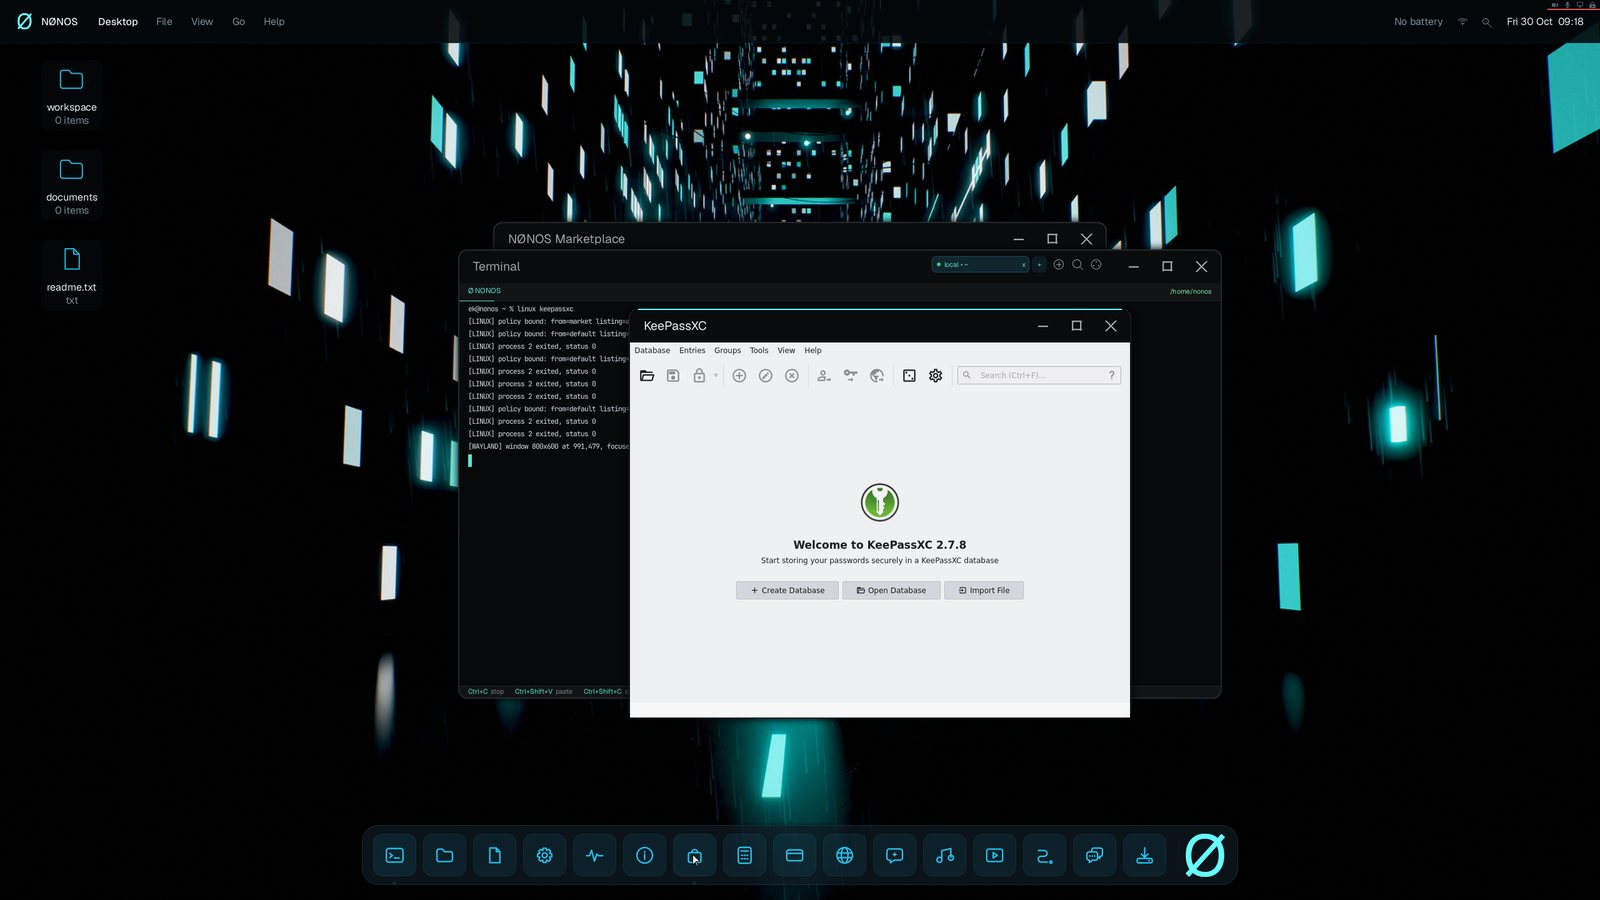
\includegraphics[width=0.82\textwidth]{figures/keepassxc-in-its-box.jpg}
\caption{KeePassXC 2.7.8, a Linux password manager, drawing its own window on the \nonos{} desktop, with the Terminal that started it behind it showing \code{[LINUX] policy bound} lines. Its box is \code{WAYLAND} and \code{FILES\_HOME}: a window and a home folder, no network. Sealed 0.9.3 image under KVM. The screenshot shows a welcome screen; it does not show a database being made or opened.}
\label{fig:keepass}
\end{figure}

\subsection{Terminals}

A terminal emulator opens a pseudo-terminal before it starts a shell, and until 0.9.3 there was none to open. A guest can now open \code{/dev/ptmx}, and \code{/dev/pts/N} opens the slave once it is unlocked. A family holds at most 64 pairs. What the master writes passes the slave's line discipline: input mapping, \code{\string^C} as a signal for the foreground group under \code{ISIG}, line editing under \code{ICANON}, echo. A changed window size raises \code{SIGWINCH}. When the master goes, the slave reads end of file and its session leader gets \code{SIGHUP}.\note{\path{docs/userland/linux-personality.md}, section "Pseudo-terminals"; \path{userland/capsule_linux/src/linux/pty/table.rs:25-50}.} A master writing with no reader stops at 4,096 pending bytes or lines and 64~KiB of output.\note{\path{docs/release/0.9.3-what-is-new.md}, section "Pseudo-terminals".} foot ran a shell over \code{/dev/pts} on a development image. That is the one booted use we can point to.\src{docs/release-evidence/0.9.3/gui-foot/README.md}

\subsection{The thirty-one programs}

Table~\ref{tab:programs} lists the catalogue as it stands in the tree: 31 entries, each with its box and licence. One of them, the SimpleX Chat core, is an engine for a window that is not in this release and is not meant to be run directly, so 30 are things a person starts. The release notes count 30 recipes for that reason, and the README counts 31 rows.\note{\path{userland/capsule_market/linux-catalogue.json}; \path{docs/release/0.9.3-what-is-new.md}, section "The Marketplace".}

Two features of the table are worth reading before the table. First, every program holds \code{FILES\_HOME}, and no program holds the person's files: the box for a text editor is a terminal and its own empty home. Second, only eight programs hold \code{NET\_ANON}, and the ones that do are chat clients, wallets and Telegram. The shipped listings name no destinations, so a program with \code{NET\_ANON} may open a stream to any host and port over the chosen route. A destination list is part of the policy format, and \code{linux --box} accepts one, but the catalogue uses it for none of its entries.\src{userland/capsule_market/linux-catalogue.json}

\begin{table}[t]
\centering
\caption{The \nPrograms{} programs in the Marketplace catalogue with their boxes, grouped by what they draw. Generated from \code{userland/capsule\_market/linux-catalogue.json} by \code{paper/tools/gen\_tables.py}. Twenty-five come from Alpine v3.20 packages. The other six are not Alpine packages: DarkFi's four are built from source at a pinned commit, and SimpleX's two are the upstream release binary pinned by hash. A listing in this table is not evidence that the program has run: the status of each is in Section~\ref{sec:status}.}
\label{tab:programs}
% generated by paper/tools/gen_tables.py from linux-catalogue.json
{\footnotesize\setlength{\tabcolsep}{4pt}
\begin{longtable}{@{}>{\raggedright\arraybackslash}p{3.6cm}>{\raggedright\arraybackslash}p{6.6cm}>{\raggedright\arraybackslash}p{4.2cm}@{}}
\toprule Program & Its box & Licence\\ \midrule\endhead
\multicolumn{3}{@{}l}{\textit{With a window of their own} (7)}\\
swayimg & \texttt{WAYLAND FILES\_HOME} & MIT\\
Telegram Desktop & \texttt{WAYLAND FILES\_HOME NET\_ANON} & GPL-3.0-or-later + exc.\\
KeePassXC & \texttt{WAYLAND FILES\_HOME} & GPL-2.0-only OR GPL-3.0-only\\
foot (terminal) & \texttt{WAYLAND TTY FILES\_HOME EXEC} & MIT\\
mpv (media player) & \texttt{WAYLAND FILES\_HOME} & GPL-2.0-or-later\\
zathura (PDF viewer) & \texttt{WAYLAND FILES\_HOME} & Zlib\\
DarkFi (chat app) & \texttt{WAYLAND FILES\_HOME NET\_ANON} & AGPL-3.0-only\\
\addlinespace
\multicolumn{3}{@{}l}{\textit{In the Terminal} (23)}\\
Helix & \texttt{TTY FILES\_HOME} & MPL-2.0\\
micro & \texttt{TTY FILES\_HOME} & MIT\\
Kakoune & \texttt{TTY FILES\_HOME EXEC} & Unlicense\\
Vim & \texttt{TTY FILES\_HOME} & Vim\\
bat & \texttt{TTY FILES\_HOME EXEC} & Apache-2.0\\
eza & \texttt{TTY FILES\_HOME} & MIT\\
nnn & \texttt{TTY FILES\_HOME EXEC} & BSD-2-Clause\\
ncdu & \texttt{TTY FILES\_HOME} & MIT\\
fzf & \texttt{TTY FILES\_HOME EXEC} & MIT\\
Git & \texttt{TTY FILES\_HOME EXEC} & GPL-2.0-only\\
tig & \texttt{TTY FILES\_HOME EXEC} & GPL-2.0-or-later\\
lazygit & \texttt{TTY FILES\_HOME EXEC} & MIT\\
age & \texttt{TTY FILES\_HOME} & BSD-3-Clause\\
minisign & \texttt{TTY FILES\_HOME} & ISC\\
FLAC & \texttt{TTY FILES\_HOME} & BSD-3-Clause AND GPL-2.0-or-later\\
LAME & \texttt{TTY FILES\_HOME} & LGPL-2.0-or-later\\
Geth (dev chain) & \texttt{TTY FILES\_HOME NET\_LISTEN\_LO} & GPL-3.0-or-later\\
Profanity (XMPP, OMEMO) & \texttt{TTY FILES\_HOME NET\_ANON} & GPL-3.0-or-later\\
Monero wallet (CLI) & \texttt{TTY FILES\_HOME NET\_ANON} & BSD-3-Clause\\
DarkFi wallet (drk) & \texttt{TTY FILES\_HOME NET\_ANON} & AGPL-3.0-only\\
DarkFi local dev chain & \texttt{TTY FILES\_HOME NET\_LISTEN\_LO JIT} & AGPL-3.0-only\\
DarkIRC (P2P chat) & \texttt{TTY FILES\_HOME NET\_ANON NET\_LISTEN\_LO} & AGPL-3.0-only AND MIT\\
SimpleX Chat (terminal) & \texttt{TTY FILES\_HOME NET\_ANON} & AGPL-3.0-only\\
\addlinespace
\multicolumn{3}{@{}l}{\textit{A background engine} (1)}\\
SimpleX Chat core & \texttt{FILES\_HOME NET\_ANON} & AGPL-3.0-only\\
\bottomrule
\end{longtable}}

\end{table}

\subsection{What the kernel refused}

We ran Linux programs on the sealed 0.9.3 image under KVM and tried the things a hostile program would try. Figure~\ref{fig:refusals} is the Terminal after three of them, and Table~\ref{tab:refusals} lists six, each with the answer the system gave.

\begin{figure}[t]
\centering
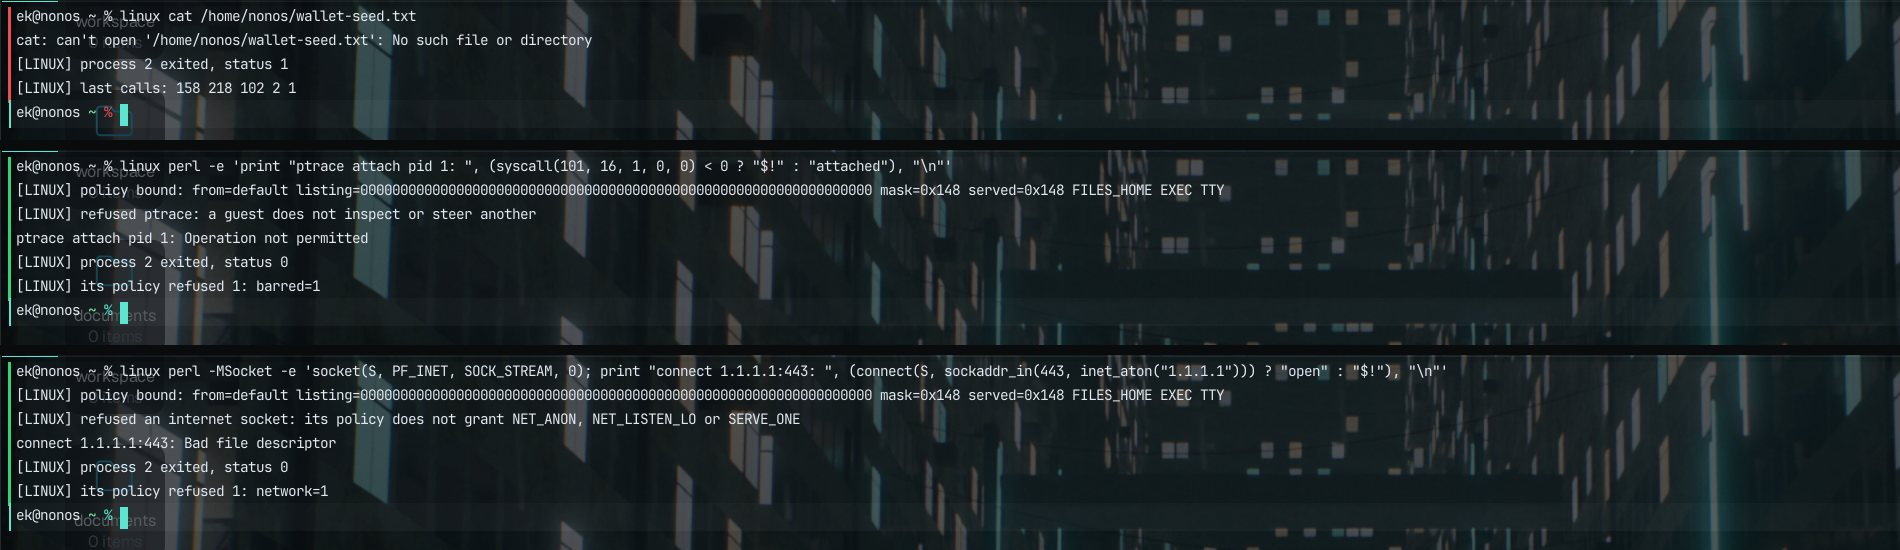
\includegraphics[width=\textwidth]{figures/refusals.jpg}
\caption{The Terminal after three attempts from inside a Linux program: reading a file that is not in its world, attaching with \code{ptrace} to process 1, and opening an internet socket and connecting out. The \code{policy bound} lines show \code{from=default}, a listing of all zeros and \code{mask=0x148}, which is \code{FILES\_HOME}, \code{EXEC} and \code{TTY}: the default box of a program typed at the Terminal with no listing. Sealed 0.9.3 image under KVM, no TPM. Single attempts, as the next paragraph says.}
\label{fig:refusals}
\end{figure}

\begin{table}[t]
\centering
\caption{Six attempts from inside a Linux program on the sealed 0.9.3 image, and what the system answered. The first three are in Figure~\ref{fig:refusals}. The other three come from the project's README table of the same run, whose screenshot we do not have. The fourth, the refused \code{execve}, needs a box without \code{EXEC}, so it was not run in the default box of the figure.}
\label{tab:refusals}
\footnotesize
\begin{tabular}{@{}>{\raggedright\arraybackslash}p{3.3cm}>{\raggedright\arraybackslash}p{11.2cm}@{}}
\toprule Attempt & Answer\\ \midrule
Read the person's files & \code{cat: can't open '/home/nonos/wallet-seed.txt': No such file or directory}; its \code{/home} is empty\\
Attach to another process & \code{[LINUX] refused ptrace: a guest does not inspect or steer another}\\
Open a connection out & \code{[LINUX] refused an internet socket: its policy does not grant NET\_ANON, NET\_LISTEN\_LO or SERVE\_ONE}\\
Start another program & \code{[LINUX] refused execve: its policy does not grant EXEC}\\
See other programs & \code{ls /proc} shows one process, its own\\
Read the keyboard & \code{cat /dev/input/event0}: no such device\\ \bottomrule
\end{tabular}
\end{table}

These are single attempts from inside an app. They are not an exploit chain, and nobody has tried one. A program that is granted a right is allowed it: Telegram's box gives it the network, and it uses the network. We do not claim the box cannot be broken. What the attempts show is narrower and, to us, still worth having: the refusals are specific, they name the missing word, and they come from the code paths in Section~\ref{sec:box} that we can point to.

A second, earlier suite is committed with its serial log. A Perl script on a development image tried what a hostile app would: \code{ptrace} and \code{process\_vm\_readv} on process 1, a kernel module load, \code{kexec}, \code{mount}, an anonymous mapping that is both writable and executable, a one-terabyte mapping, a mapping made executable after the fact, signals to every pid, \code{/proc/kcore} and \code{/dev/mem}, a TCP connect and a UDP send with no network word, a raw socket, and a fork loop. Each was refused or bounded; the fork loop stopped at 511, the family's ceiling. That boot was under QEMU's software emulation, on a branch with one extra system call that this release does not carry, and the first attempt at it was thrown away because Perl's \code{syscall} took the wrong argument.\src{docs/release-evidence/0.9.3/s1-isolation-61ec29ea2/README.md} We include the failed attempt because it is the usual way such a test goes wrong.

The kernel's side of the story is visible in the \code{audit} command, shown in Figure~\ref{fig:audit}. It lists every process with the reach its capability word gives it (network, storage, devices, launch), who signed it and every bit it holds. Kernel threads show as not in the registry, with no signed ceiling recorded.\src{userland/capsule_terminal/src/command/builtin/audit/table.rs:16-66}

\begin{figure}[t]
\centering
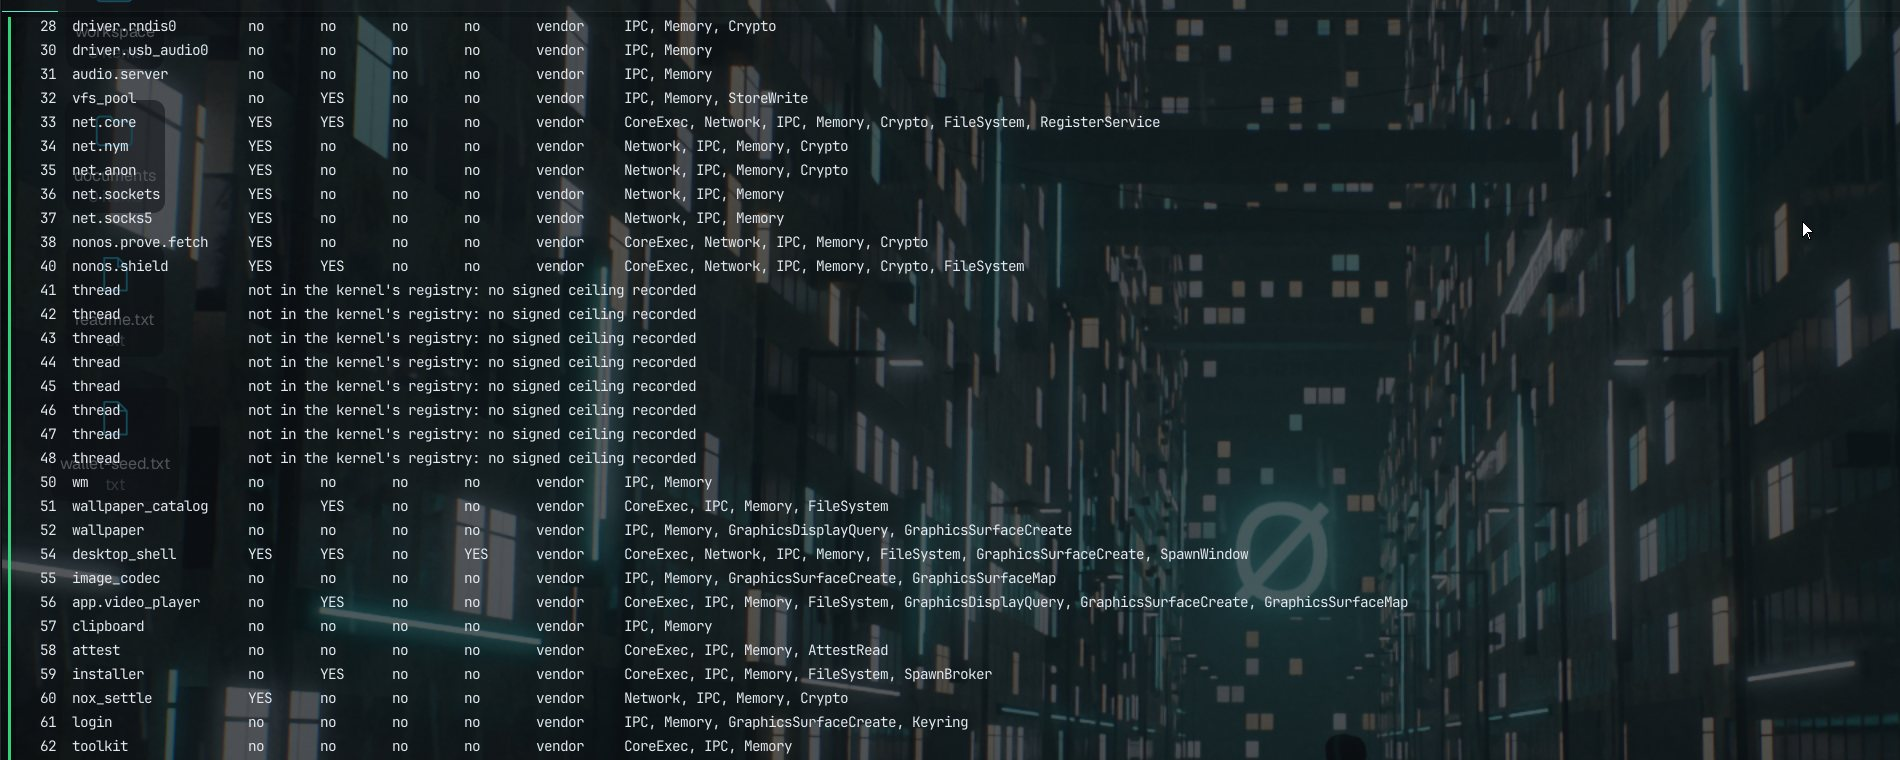
\includegraphics[width=\textwidth]{figures/audit.jpg}
\caption{Part of the \code{audit} table on the sealed 0.9.3 image under KVM. Columns after the name are four reach areas (network, storage, devices, launch), the signer (\code{vendor} for every row shown) and the capability bits the process holds. Rows 41 to 48 are threads, which have no signed ceiling. The \code{devices} column names capability bits the kernel would honour, not devices claimed at the moment.}
\label{fig:audit}
\end{figure}

\subsection{Running a program you wrote, or a model did}

The same machinery is available by hand. \code{linux --box} runs a program in a named box and prints a report of what the box refused:

\begin{verbatim}
linux --box strict sh -c 'echo ok > /tmp/out; echo no > /home/out; nc 10.0.0.1 80'
linux --box offline python3 script.py
linux --box allow:/tmp/out,net:api.example.com:443 python3 agent.py
\end{verbatim}

\code{strict} has no network and writes only to \code{/tmp}. An \code{allow:} box names its folders and, if it needs any, its destinations. A connection anywhere else is refused and counted, and the destination list is the one place in the current tree where a box can name hosts. \code{linux --box learn} runs a program once, enforced as \code{offline}, and writes the tightest box file that would have let it do what it did. The file is one run's behaviour, not what the program may need on another, and the documentation says to read it before use.\src{docs/using/linux-box.md} The report's counts are made by the personality as it refuses; they are not the kernel's histogram, and the page says so. This is the use we expect from people who run code a model wrote: a throwaway box, a printed list of what it tried, a file to tighten next time.

\subsection{Where the box is weak}\label{sec:box-limits}

The box is a design with a working implementation, not a finished wall, and we would rather say where it is thin than wait for someone else to.

\textbf{The call set does not narrow anything yet.} A recipe without a measured set is \emph{unmeasured}: buckets 0 to 511 set and 512 clear, so every Linux call is allowed and only the native bucket is barred. None of the 31 catalogue entries carries a measured set. The machinery to enforce a narrower one exists and is tested on the host, and a listing could use it, but the boxes in Table~\ref{tab:programs} are, in practice, the mask plus the seventeen calls refused on purpose.\note{\path{docs/userland/marketplace-catalogue.md}, section "The recipes file"; \path{userland/nonos_linux_policy/src/market.rs:31-43}.}

\textbf{The box is kept by path.} The catalogue documentation lists three ways around it that are open today: a listed package's dependencies install unheld and run in the default box (tig pulls git, bat pulls less, vim pulls xxd); a held program copied to another path along with its trailer; and the loader invoked as \code{/lib/ld-musl-x86\_64.so.1 <program>}, because the loader's gate checks only the trailer. Each ends in the default box, with every call allowed and no network. The proposed fix, tying a policy to the program's hash and not its path, is not in this release. We rely on that page at this commit; we did not re-run the three.\note{\path{docs/userland/marketplace-catalogue.md}, section "What a listing carries".}

\textbf{The supervisor is a large target.} It holds \code{FileSystem}, \code{Crypto}, \code{StoreWrite}, \code{ForeignExec} and \code{Debug} at all times, and the threat model says that authority follows the process, not the code. A program that takes over the personality gets those bits. One personality instance serves a run's guests together, a program and everything it starts. The personality's own documentation reports 369 host tests passing in the flake checks; the Linux surface is still a large amount of code to hold to a policy.\note{\path{docs/security/protections-and-limits-what-nonos-does.md}; \path{docs/userland/linux-personality.md}, section "Tests".}

\textbf{A home does not survive power-off.} A Linux program's home is held in memory, at most 16~MiB (64~MiB for the Monero wallet) and 128 names, and is gone at power-off. A home kept across a reboot is designed and not in the release, so the only lasting copy of a wallet seed is the one written down.\note{\path{userland/capsule_linux/src/linux/file/system/declared/home.rs:29-32}; \path{docs/release/0.9.3-known-issues.md}, section "Linux apps".} The design page says in its first line that kept homes move to the next release.\src{docs/design/kept-homes-and-installs.md}

\textbf{The proof of a run has not completed on a boot.} The Marketplace's proof of how a program ran timed out in two boots, and the 180-second wait that followed is not booted. Programs also fail in ways the tree states plainly: \code{lame} ended on signal 11 on a development boot, \code{micro} opened from the Marketplace stops on \code{open /dev/tty}, and \code{age}'s passphrase prompt, which writes to \code{/dev/tty}, does not show.\note{\path{docs/release/0.9.3-known-issues.md}, section "Linux apps".}

\textbf{Nobody outside the project has attacked it.} The refusals above were produced by us, against our own code, on images we built. That is not an audit.

\section{Cryptography}\label{sec:crypto}

\subsection{Signatures}

Key files, certificates and manifests name the algorithm of each key in one byte: Ed25519, ML-DSA-44, ML-DSA-65 or ML-DSA-87. The kernel verifies only Ed25519 and ML-DSA-65, and the signer produces only those two.\src{src/crypto/asymmetric/alg_id/verify.rs:23-42} ML-DSA-65, a FIPS~204 parameter set \cite{fips204}, comes from PQClean's portable C code under \code{third\_party/pqclean}.\src{build.rs:229-235} Requiring both algorithms means a forger must break both: Ed25519 against classical attackers and ML-DSA-65 against one with a quantum computer. The boot-root record and the kernel approval are signed with an ECDSA P-256 device-policy key. The kernel checks the record. The TPM checks the approval itself before it releases the device secret, and P-256 is a curve the TPM can verify. That key is not post-quantum, and we say so.\note{\path{docs/security/boot-chain-and-signatures.md}, section "Keys and where their public halves live".}

Sizes: an Ed25519 public key is 32 bytes and its signature 64; an ML-DSA-65 public key is 1,952 bytes and its signature 3,309.\src{src/crypto/asymmetric/alg_id/lengths.rs:19-26} A manifest with both signatures therefore spends most of its bytes on the post-quantum one, and we think that is the right trade for a signature checked once at spawn.

\subsection{Hashes and the STARK}

Measurements use BLAKE3. The STARK layer uses Poseidon over the Goldilocks field for leaves and paths \cite{poseidon}, and the proof system is transparent and hash-based \cite{stark,fri}, so its security does not rest on discrete logarithms or pairings. The verifier is \code{nox\_verify} from the STARKs repository, pinned by commit; no proof in the kernel tree covers its soundness.\note{\path{Cargo.toml:1444}; \path{docs/security/stark-attestation.md}, section "What a trailer does not prove".}

\subsection{Keys the machine holds}

The kernel signs capability tokens with a 32-byte key drawn at boot.\src{src/capabilities/token/material.rs:41-52} Machine keys are derived by the TPM under PCR policy and never stored (Section~\ref{sec:chain}). Sealed records use ChaCha20-Poly1305 written in the tree, with keys from HKDF-SHA256 over the machine key and the record name.\src{userland/nonos_seal/README.md:1-12}

Three limits are documented. The TPM exchange that derives machine keys is unbound and unsalted, so on a discrete TPM the key crosses the bus in the clear. Labels are not tied to capsules, so any capsule holding \code{Crypto} can derive any machine-key label other than the kernel's own. And sealed records have no rollback protection: an older blob opens as well as a newer one.\srcs{docs/security/protections-and-limits-what-nonos-does.md}{userland/nonos_vault/README.md:32-34}

\subsection{Entropy}

0.9.2 reported that the generator serving \code{CryptoRandom} to capsules was seeded from RDRAND alone. The documentation now says otherwise, and we follow it. Both of the kernel's generators are seeded from the \code{entropy\_pool} capsule's bytes mixed with RDSEED and RDRAND, and the capsule's bytes are never counted as enough alone: a seed needs 32 bytes from RDSEED and RDRAND, of which the capsule can supply at most 16. The loader adds a 32-byte seed of its own. The TPM is not a source.\note{\path{docs/security/randomness-and-cryptography.md}, section "Sources"; \path{docs/security/randomness-when-missing.md}.}

When no hardware source answers, the behaviour is the part to read. \code{get\_bytes\_secure} fails rather than fall back, but \code{fill\_random\_bytes} falls back to the cycle counter XORed with a counter, and a kernel with no hardware source still boots.\srcs{src/crypto/random_api/basic.rs:42-46}{docs/security/randomness-when-missing.md} We have not found a check in the boot path that stops a machine with no source, and the documentation does not claim one.

\section{Networking and privacy}\label{sec:net}

\subsection{Routes}

The person chooses one of three routes in first-boot setup: the Nym mixnet, which is the default; the Anyone onion network; or Direct. One library, \code{nonos\_route\_link}, holds the rule for every program that opens its own connections. Direct is used only when Direct is chosen, Anyone goes through \code{net.anon}, and anything else, an unreadable setting included, goes through Nym. A chosen network that is not running means no route, and nothing falls back.\srcs{userland/nonos_route_link/src/pick.rs:130-139}{docs/using/privacy-network.md} The wallet's chain reads and broadcasts never go Direct: under a Direct default they go over Nym, or over Anyone when Nym is not running, and with neither up there is no route.\src{userland/nonos_route_link/src/pick.rs:86-100} Downloads for installs use Anyone whatever the default, because Nym's exits end long streams part way and Anyone's circuits carry gigabytes.\src{userland/nonos_route_link/src/pick.rs:46-60} Host names travel unresolved to the exit, so no clear DNS query leaves the machine. Network drivers draw a new locally administered MAC address at each bring-up.\srcs{docs/using/privacy-network.md}{userland/nonos_mac/src/local.rs:46-55}

\begin{figure}[t]
\centering
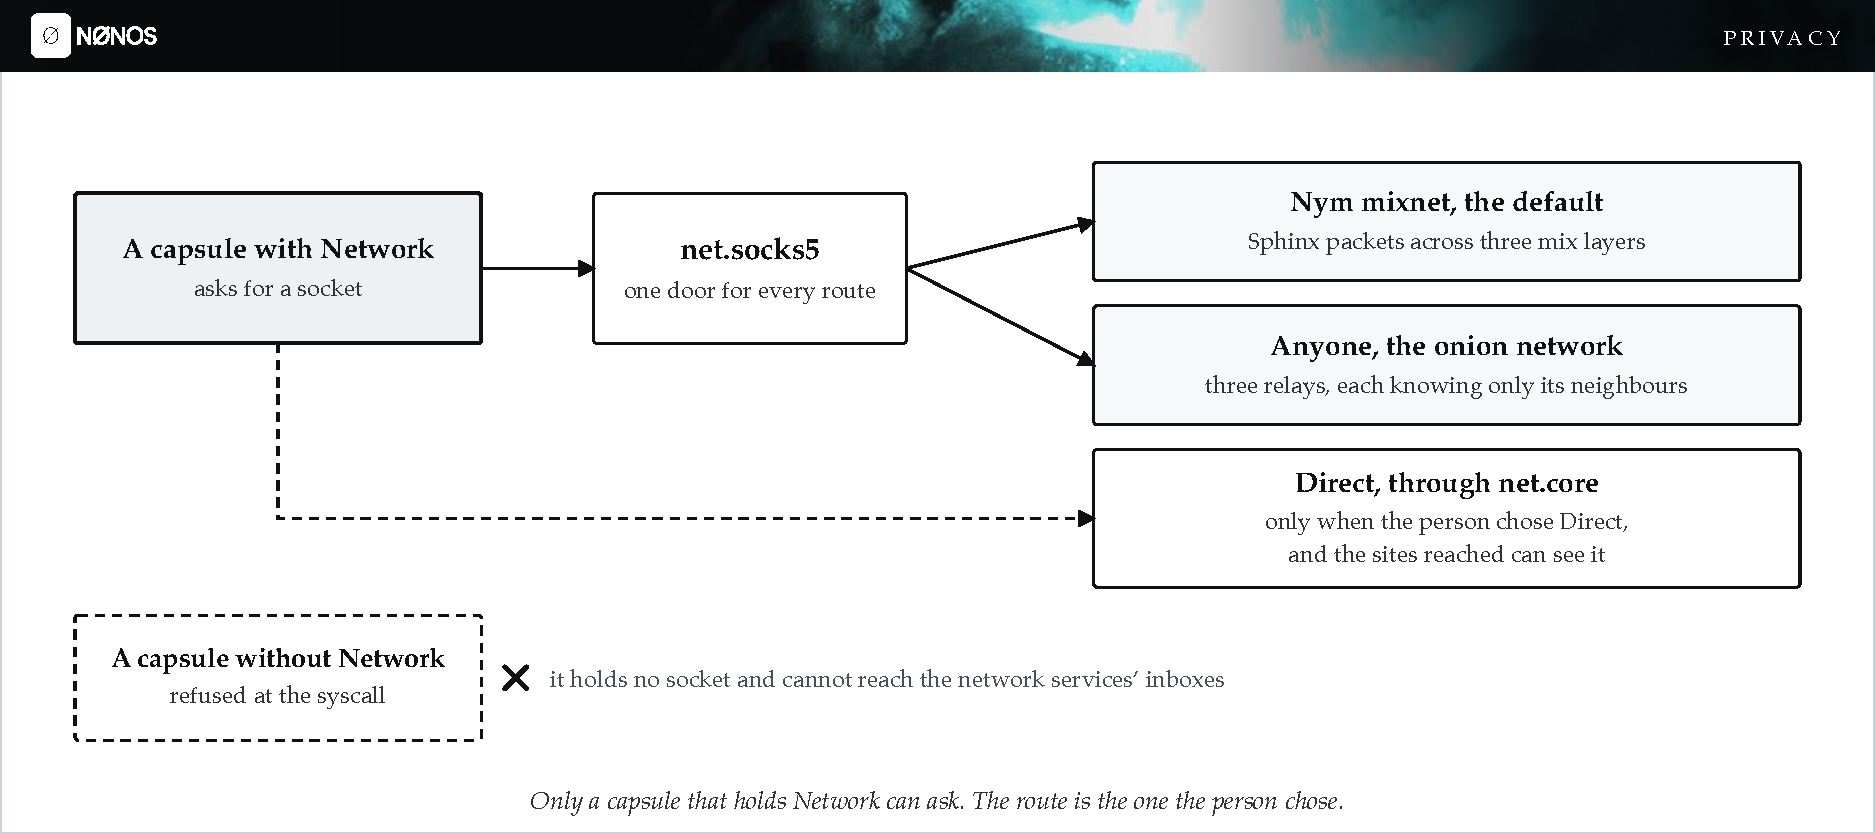
\includegraphics[width=0.84\textwidth]{figures/diagram-network-routes.pdf}
\caption{How a program's traffic leaves the machine. A capsule that holds \code{Network} asks \code{nonos\_route\_link} for a route; Nym streams go through \code{net.socks5} and \code{net.nym}, Anyone streams through \code{net.anon}, and Direct through \code{net.sockets}. A capsule without \code{Network} cannot reach the network services' inboxes. A Linux program in a box with \code{NET\_ANON} takes the same library's route and is never given Direct. Sources: \code{docs/using/privacy-network.md}, \code{src/services/registry/policy.rs}.}
\label{fig:routes}
\end{figure}

\begin{figure}[t]
\centering
\begin{minipage}[t]{0.40\textwidth}
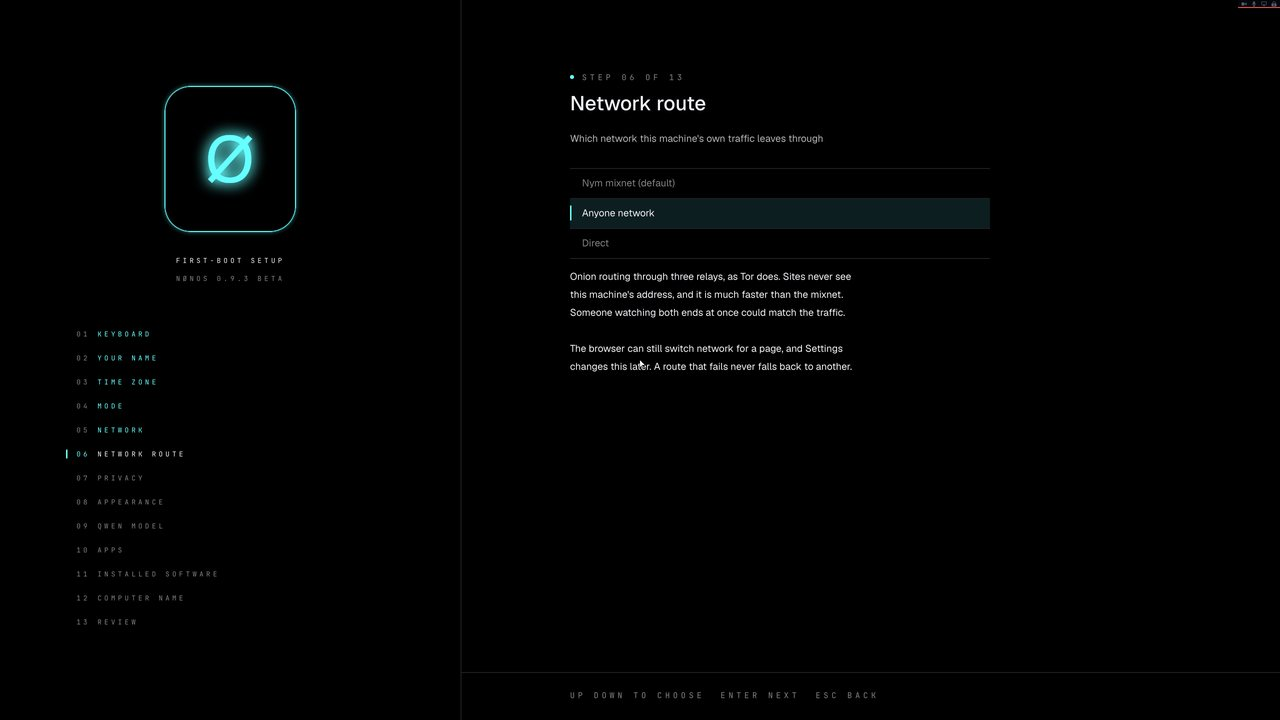
\includegraphics[width=\textwidth]{figures/setup-route.jpg}
\end{minipage}\hfill
\begin{minipage}[t]{0.40\textwidth}
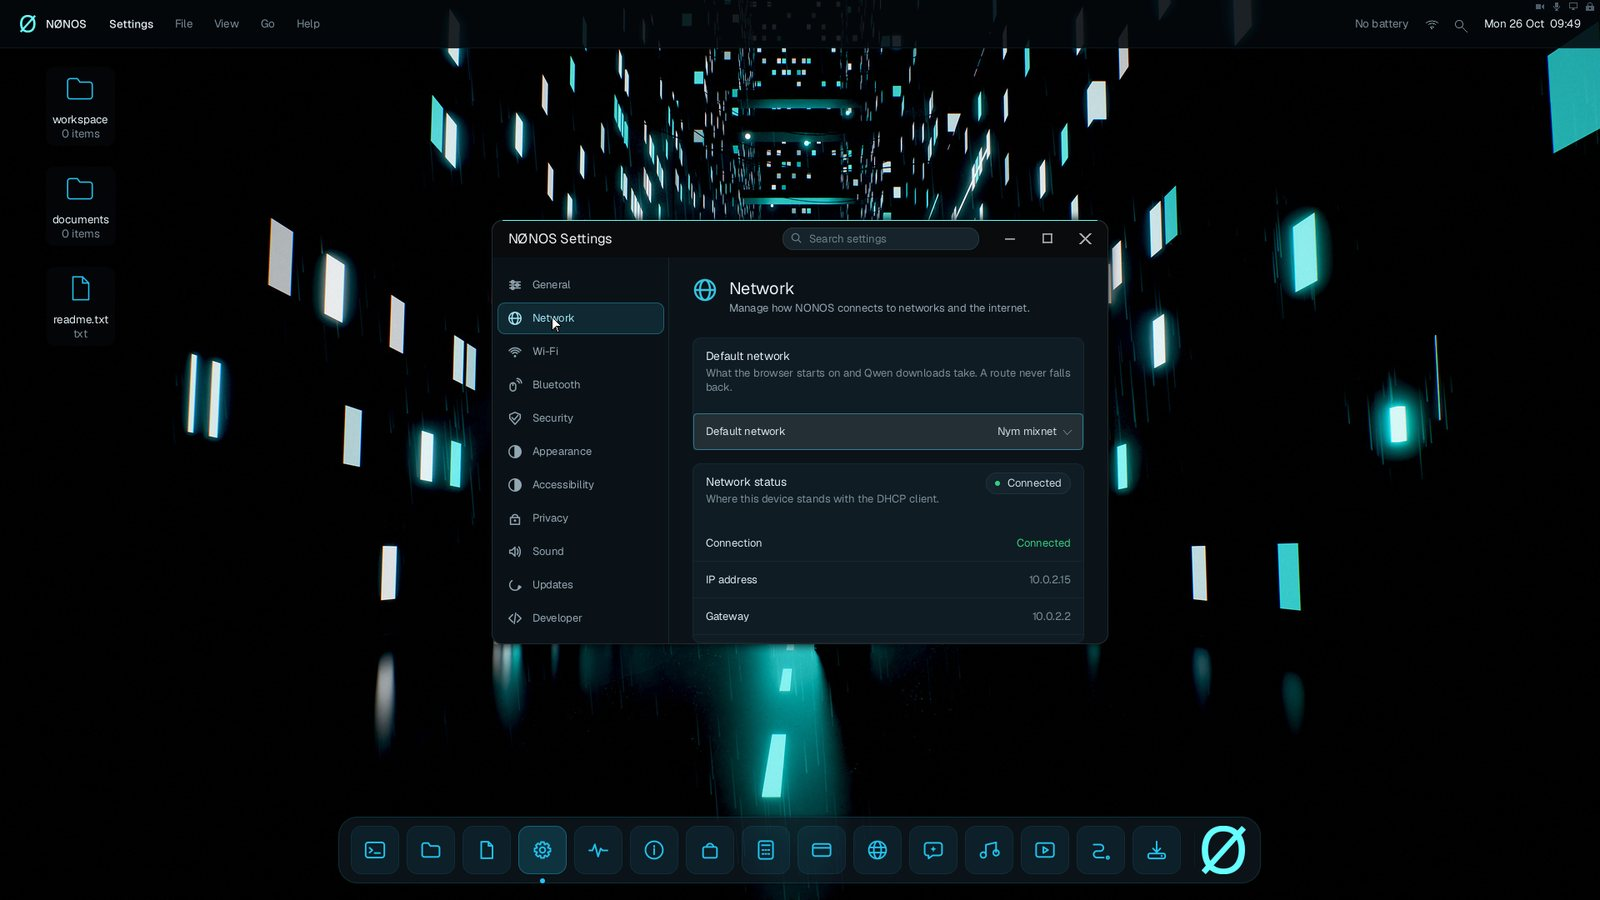
\includegraphics[width=\textwidth]{figures/settings-network.jpg}
\end{minipage}
\caption{Left, the first-boot step that picks the network the machine's traffic leaves through. Right, Settings, which shows the network in use and changes it. Both from the sealed 0.9.3 image under KVM, so Settings shows a virtual network, not a real one.}
\label{fig:routeshots}
\end{figure}

\subsection{What a Linux guest gets}

For a Linux program the route logic is the same code with one extra rule. A stream to anywhere outside the program's own family goes by the system's chosen network: Anyone to \code{net.anon}, Nym or an unreadable setting to the mixnet socket, and Direct also to the mixnet, because a guest is never given a direct socket. A chosen network that is not running is \code{ENETUNREACH}, and nothing else is tried.\src{userland/capsule_linux/src/linux/net/guest_route.rs:59-75} A program binds and listens only on 127.0.0.0/8; a datagram to outside the family is \code{ENETUNREACH}; a raw internet socket is \code{EPERM}.\src{userland/capsule_linux/src/linux/net/policy.rs:33-53}

\subsection{The transports}

Both transports are new \code{no\_std} code. \nonos{} links neither the Nym client nor a Tor or Anyone client.\src{docs/security/anonymity-transports.md} \code{net.nym} builds Sphinx \cite{sphinx} packets of 2,413 bytes for the Nym mixnet \cite{nym} with a 348-byte header across three mix layers and an exit gateway, and receives replies through single-use reply blocks. \code{net.anon} is a client for the Anyone network, a fork of Tor \cite{tor}: it checks consensus documents against directory-authority signatures, builds three-hop bandwidth-weighted circuits with the ntor handshake, and authenticates relays through Ed25519 certificates.\note{\path{docs/security/anonymity-transports.md}, section "Sphinx".} The browser, \code{curl}, \code{git} and the wallet use a \code{no\_std} TLS 1.3 client with the Mozilla root set.\src{docs/security/tls-and-certificates.md}

\subsection{What running traffic has shown}

0.9.2 had to say that no booted image had carried traffic through a live Nym gateway or Anyone circuit. 0.9.3 has some, and we say what and where.

On a KVM host, the Monero command-line wallet synced from the node named in its listing, \code{xmr-node.cakewallet.com:18081}, over Anyone and over Nym. In one Nym run the serial log counts 3,321 \code{[SOCKS5] exit answered} lines while the wallet synced; in another run a fresh wallet refreshed to 3,794,280 of 3,794,280 blocks and \code{exit} ended it with status 0. These were development images, and the install itself used the host's package relay, so the install shows nothing about the real mirror; the sync does show the route. The wallet's own window progress is quoted in the evidence from the notes of those runs, because a terminal run's output never reaches serial.\note{\path{docs/release-evidence/0.9.3/s1-g-kvm/README.md}; \path{docs/release/0.9.3-what-is-new.md}, section "The Monero wallet over Nym and Anyone".}

The same evidence is a good example of how these runs fail. An install over the real Alpine mirror stalled because the window opened three streams at once and both proxies keep one stream per caller, so each took the conversation from the one before and no package was answered. A lone stream carried the 24.7~MB Monero package whole. An install now fetches one package at a time. A failing first refresh on wallet open, "net.socks5 sent an answer this cannot read", is fixed on the host and has not been shown fixed on a boot, and the release notes tell the person to keep the seed on paper.\note{\path{docs/release-evidence/0.9.3/s1-g-kvm/README.md}; \path{docs/release/0.9.3-known-issues.md}, section "Linux apps".}

A separate capture on 25 October judged the egress of an idle first boot of a development image under QEMU. It holds 2,287 frames, 2,284 of them from the guest under one random locally administered MAC. Every peer the guest reached is pinned in the image: five Nym bootstrap gateways, Nym's directory API and seven Anyone directory authorities. There was no DNS, NTP, discovery packet or IPv6. That is the nearest thing to a test of the setup wizard's sentence, "Telemetry: NONOS has none, so there is no switch for it", and it comes with its own list of what it did not show: nobody opened an app, no relay appears in the capture, and real hardware and Wi-Fi are not covered.\note{\path{docs/security/privacy-guarantees.md}, section "Booted evidence"; \path{userland/capsule_setup_wizard/src/render/screens/privacy.rs:18}.}

\subsection{What the network design does not cover}

The kernel does not enforce the route in general. A capsule holding \code{Network} could call the TCP or socket services directly, and programs built on the toolchain's Rust \code{std} connect directly. Both transports start on every boot that starts networking, so the local network can see that a machine runs Nym and Anyone under every choice, including Direct.\src{docs/release/0.9.3-security-limits.md} Nym's directory is fetched over TLS from one validator without an operator signature, and cover traffic is sent only on request, which no program sets. \code{net.anon} has no vanguards, no conflux, no congestion control and no ntor v3, and does not check the digest in a relay's SENDME. Neither transport pads traffic on its own, and neither directory fetch is anonymous.\note{\path{docs/security/anonymity-transports.md}, section "What the transports lack".} The documentation page for the transports still says that no booted image has carried live traffic, which the evidence above contradicts; we follow the evidence and have noted the page for correction.\note{\path{docs/security/anonymity-transports.md}, section "What each transport reports".}

For Linux programs the position is better, because the route is enforced by the personality for guests and by the kernel for the instance that serves them (Section~\ref{sec:box}). For capsules in general it is a shared library and a convention that the capsules that hold \code{Network} follow.

\section{Verification}\label{sec:verify}

\nonos{} uses four kinds of evidence. Each means something different, and we keep them apart.

\subsection{Lean 4 models, and how tightly they bind to the code}

\code{verification/lean} holds 193 Lean files under Lean 4 \cite{lean4} v4.15.0 without mathlib. A count of declarations introduced by \code{theorem} or \code{lemma} finds 1,519. Counting only plain top-level \code{theorem} lines gives 1,503, which is the figure recorded in \code{verification/evidence/EVIDENCE.json}; the README says 1,517. The three numbers come from three counting rules over the same files, and we use the widest. No \code{sorry} appears outside comments in any Lean tree, which we checked by search, and the core corpus declares no axiom beyond Lean's standard \code{propext}, \code{Classical.choice} and \code{Quot.sound}; the project's CI job fails on \code{sorryAx}.\srcs{verification/evidence/EVIDENCE.json}{verification/lean/AxiomProfile.lean:1-20} We did not rebuild the proofs.

A separate tree, \code{verification/extraction}, holds about 2,200 further theorem declarations by the same widest rule, about functions that Charon and Aeneas \cite{aeneas} lowered from real Rust. EVIDENCE.json counts 978 extracted functions with 492 carrying a property of behaviour and 486 carrying only the theorem that a generated wrapper equals the method it forwards to. Eleven theorems there use \code{bv\_decide}, which adds a generated axiom that asserts a SAT certificate checker, run as compiled code, answered correctly. The record says so, and says it never reaches the core corpus.\src{verification/evidence/EVIDENCE.json}

What a theorem says about the running kernel depends on how the model is tied to the Rust. \code{verification/lean/REFINEMENT.md} defines three levels (Table~\ref{tab:levels}) and states that a level 3 entry "is not a claim about the code". Only the capability modules sit at level 1.\src{verification/lean/REFINEMENT.md} Isolation, the capability table and dispatch, the IOMMU and the wipe at power-off are proved about models at level 3, with a proof crate or an extraction for some of their parts. The README's summary says Lean "proves no reachable state reaches off without" the wipe; that is a theorem about a model of the power-off path, and the reader should hear it that way.

\begin{table}[t]
\centering
\caption{Binding levels of the Lean modules, from \code{verification/lean/REFINEMENT.md}.}
\label{tab:levels}
\begin{tabular}{@{}ll>{\raggedright\arraybackslash}p{8.2cm}@{}}
\toprule Level & Name & Meaning\\ \midrule
1 & extraction & the Rust is translated to Lean by Aeneas and the model is proved to refine it\\
2 & differential & a proof crate includes the real Rust by \code{\#[path]} and checks it against the model by tests and Kani\\
3 & specification & the model is checked in Lean; there is no mechanical tie to the Rust yet\\ \bottomrule
\end{tabular}
\end{table}

\subsection{Host proof crates, Kani and fuzzing}

The tree has 223 directories ending in \code{\_proofs} with a \code{Cargo.toml}, up from 56 at the 0.9.2 changelog. They mount shipped kernel or capsule source with \code{\#[path]} and test it with \code{cargo test} on the host. EVIDENCE.json counts 222 as runnable; we have not found which of the 223 it leaves out.\src{verification/evidence/EVIDENCE.json} There are 120 \code{\#[kani::proof]} harnesses in the tree, 115 under \code{userland/} and five in the loader and attestation crates. Kani \cite{kani} runs in a separate workflow from the flake checks.\src{docs/contributing/tests-and-proofs.md} Test counts the documentation quotes, for example 388 for \code{kernel\_proofs}, 198 for the in-tree \code{stark\_proofs} and 369 for the Linux personality's pure modules, are the documentation's, from the flake checks recorded at its own commits; we did not rerun them.\note{\path{docs/security/capsule-isolation-the-linux-personalitys.md}; \path{docs/security/stark-attestation.md}, section "Tests".}

\subsection{Static checks and adversarial tests}

Python checkers hold the published ABI to the kernel: one compares the gate of each system call, one the capability bits, one each capsule's mask against the calls its code makes.\src{scripts/check_syscall_caps.py} An attack capsule, \code{userland/capsule\_attack}, tries every row of the isolation matrix with raw system calls; no image carries it. A selftest image, which boots a capsule that tries what an attacker would, reported \code{attack suite: PASS} on a development image under QEMU, including a refused attempt to use the shell's open-with path as a deputy.\srcs{docs/overview/threat-model-assets.md}{docs/release-evidence/0.9.3/ksec-d2a9d0bfa-iommu-intel/README.md}

\subsection{Reproducible builds and receipts}

The build is pinned by hash and runs offline in Nix's sandbox. \code{make} ends with a receipt of every artifact by SHA-256 and prints \code{REPRODUCED} when the bytes match the committed receipt.\src{receipts/README.md} Sealed images differ by design, because signatures and trailers differ between seals. A comparison of builds on two machines is not tested in this release, and the documentation lists what is not reproducible yet.\src{docs/build/reproducible-builds.md}

\subsection{What has not run}

Several checks that matter for the trust path did not run for this release. No flake check runs \code{nox\_verify} over a real proof; the enrolment tool's selftest does, and no run of it is recorded for this commit. The booted refusal test, which expects four STARK refusals and one admission under QEMU, was not run. The Kani harnesses for the attestation path crate were not run. The Marketplace's proof of how a program ran has not finished on a boot. And the claims in Section~\ref{sec:box} about the box rest on boots of development images and one sealed image, not on a proof.\note{\path{docs/security/stark-attestation.md}, section "Tests"; \path{docs/release/0.9.3-known-issues.md}.}

The public verifier at \code{verify.nonos.software} runs \code{nox\_verify} compiled to WebAssembly over the 0.9.2 release's enrolled units. We did not check what it lists for 0.9.3, and this paper does not rely on it.

\section{The Ethereum angle}\label{sec:eth}

This section separates what exists from what is a direction. Nothing in it describes a shipped product for machine attestation on Ethereum. It is shorter than in 0.9.2, because the kernel repository holds no Solidity and nothing in this release moved the direction forward. We keep it because the question is why the project started, and because the box of Section~\ref{sec:box} sharpens it.

\subsection{The weak link}

Ethereum secures its state with consensus and with code that every node executes. The machines at its edges are outside that guarantee. A wallet machine that runs a compromised program can sign whatever the program asks. A validator's signing key is only as safe as the server that holds it. An RPC provider sees which accounts a given network address asks about, and that links a person's location to their holdings. A contract can check a signature. It cannot learn anything about the machine that produced it.

The box adds a smaller point. A wallet that reads a seed from a file is only as private as every program that can read that file. In \nonos{} a program in a box has no access to the person's files at all. That is a property of the endpoint, and no on-chain rule can see it.

\subsection{What exists today}

\begin{figure}[t]
\centering
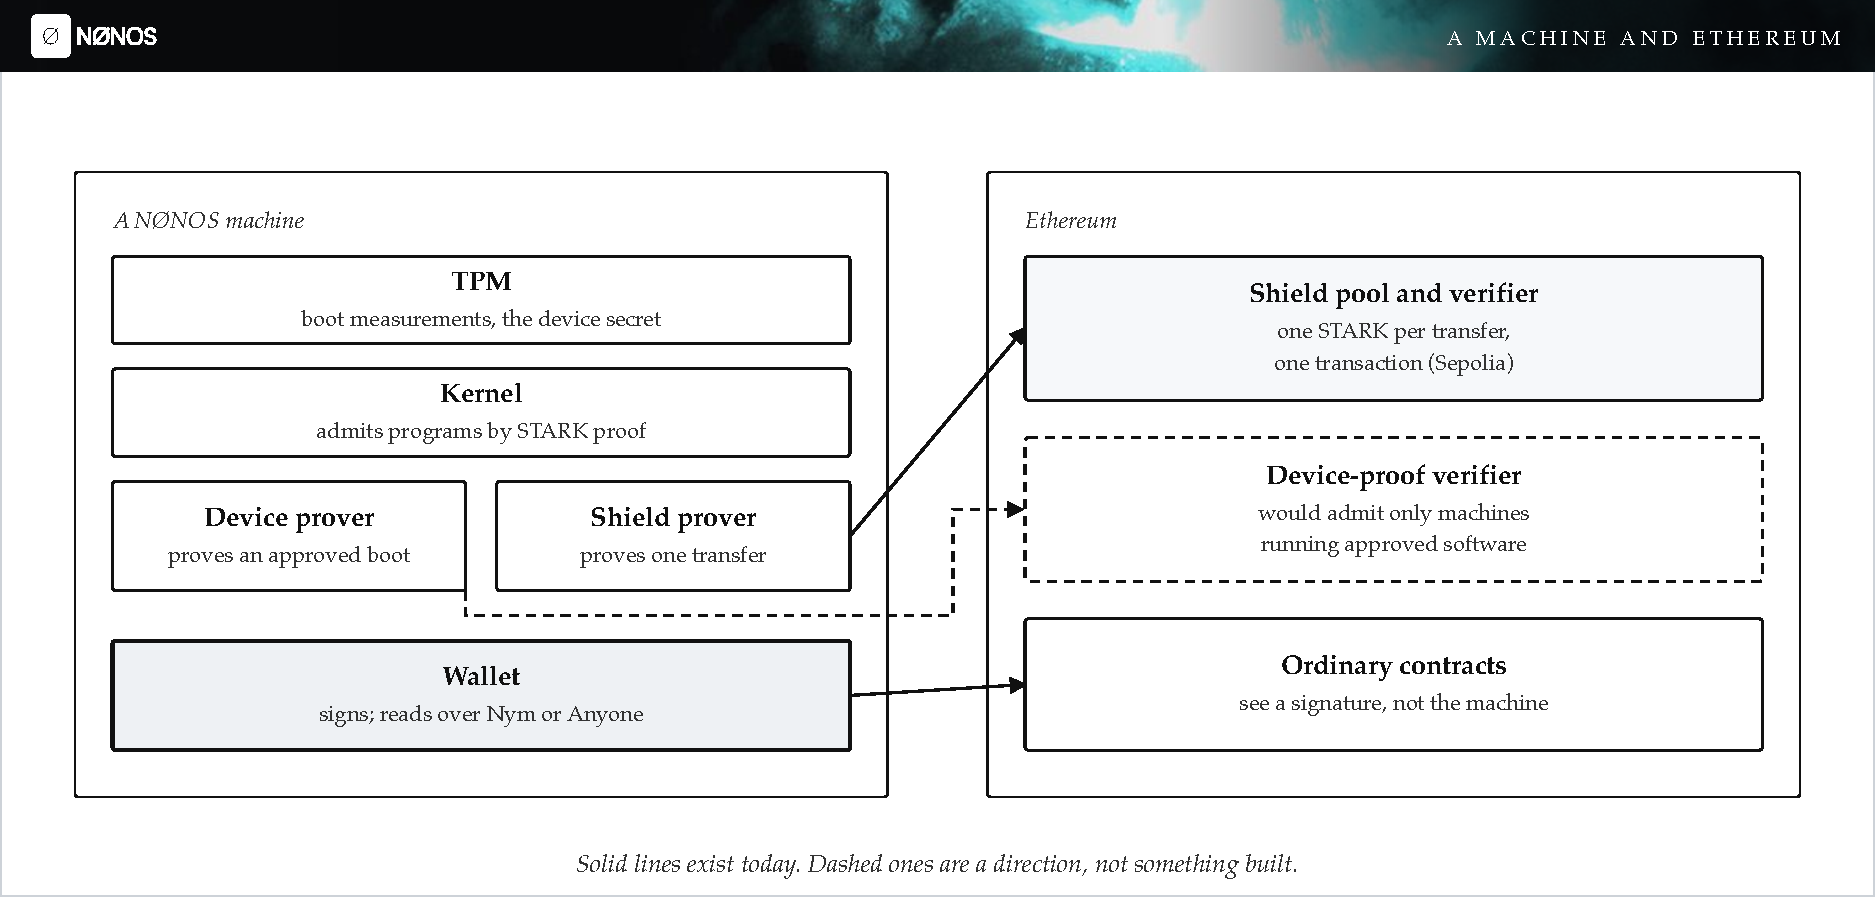
\includegraphics[width=0.84\textwidth]{figures/diagram-machine-and-ethereum.pdf}
\caption{What connects a \nonos{} machine to Ethereum, and what does not exist yet. Solid lines exist today; dashed ones are a direction, not something built. Sources: \code{docs/security/stark-attestation.md}, \code{nonos-device-attest/README.md}, \code{abi/NOX\_CONTRACTS.md}.}
\label{fig:eth}
\end{figure}

A \nonos{} machine can produce proofs about itself. Three artefacts exist, all checked off-chain. The admission proofs: every enrolled kernel, loader and capsule carries a STARK of membership under a public root. The TPM quote from \code{MkAttestDoc}, which names the machine and is withheld from any capsule with network rights. And the anonymous device proof of Section~\ref{sec:chain}, whose own README lists it as built and never run on a booted image, and which no verifier service or contract consumes.\srcs{docs/security/stark-attestation.md}{nonos-device-attest/README.md}

The wallet hides the RPC link. The wallet's chain reads go over Nym or Anyone, with host names resolved at the exit, and never over Direct (Section~\ref{sec:net}).

The NOX token has a contract set specified in the tree. \code{abi/NOX\_CONTRACTS.md} describes a contributor-reward system: off-chain receipts for work such as boots and capsule builds, aggregated into Merkle roots and paid from reward pools, with a deployment record on Ethereum mainnet under a 3-of-5 Safe. We did not query the chain to confirm the deployment, and the Solidity is not in this repository. The page is explicit that "v1 verification is off-chain with open tooling" and that v1 does no on-chain ZK verification. In 0.9.2 the same page listed ten contracts; it now lists eight, and we report it as the document stands.\srcs{abi/NOX_CONTRACTS.md}{abi/nox_deployment.json}

The Shield pool, which settles a private transfer with one STARK checked by a verifier contract, is described in a separate paper \cite{shield} and in repositories that are not part of this tree. We cite it and make no claim about it that we checked here. Its authors state that it has not been audited.

\subsection{What does not exist}

No contract verifies anything about a machine. No deployed contract checks an admission proof, a TPM quote or a device proof, and no transaction signature produced on \nonos{} is bound to an attested state. The project's public plan lists attested clients as an on-chain fact under work it is not building.\src{https://nonos.software/roadmap/}

\subsection{The direction}

The pieces suggest a path to a machine that proves to a contract what it runs. We state the steps and what each would need, without claiming any.

\begin{enumerate}
\item A verifier contract for the device proof. It proves a different statement over a different trace from the Shield pool's, so it would be a new contract with its own gas cost and its own audit.
\item Roots on chain: the release's bootloader, kernel and device-registry roots, from a source a contract trusts, such as a registry updated by the release's multisig.
\item Scope and freshness. The statement already binds a verifier scope and a nonce and yields one tag per device per scope, so a contract could use its own address as the scope and a recent block hash as the nonce.
\item Binding an action to the proof. The statement has no field for a public key or a message, so letting a contract accept a signature only from an attested machine would change the circuit.
\end{enumerate}

Two limits would remain. The proof shows that an approved chain exists and that the prover holds an enrolled device secret; that this machine booted that chain rests on the TPM releasing the secret only in that boot state, and so on the TPM and firmware being honest. And the proof says nothing about the behaviour of the code it admits, only its identity. Section~\ref{sec:box} is the other half of that sentence: identity of the system's own code from the proof, behaviour of everyone else's from the box. A contract that wanted to know that the signing machine could not be reached by a stray program would need both.

\section{Status}\label{sec:status}

Table~\ref{tab:status} gives the state of each component at the studied commit, from evidence in the tree. We use four columns. \emph{Built}: the code is in the tree and in the release artifacts. \emph{Booted}: a boot exercised it, and the cell says which kind. \emph{Hardware}: a run on physical hardware is recorded. \emph{Audited}: an external party reviewed it. No component has been externally audited. The release notes say that this release claims no third-party security audit, and the bug-bounty policy is a draft.\srcs{docs/release/0.9.3-security-limits.md}{docs/overview/mission.md}

Two kinds of boot matter and are easy to confuse. A \emph{development image} is built with throwaway keys and path-only attestation, under QEMU. Most of the more than fifty evidence directories are of that kind. A \emph{sealed image} is the release build, signed and enrolled with the release keys. The screenshots in this paper are from a sealed image under KVM, which gives the guest no TPM, so the TPM paths did not run in them.\src{docs/release-evidence/0.9.3/README.md}

\begin{table}[t]
\centering
\caption{Component status at the studied commit. "Dev QEMU" is a development image under QEMU; "sealed KVM" is the sealed 0.9.3 image under KVM, with no TPM; "swtpm" is QEMU with a software TPM. "Host" means host test suites only. Real hardware means the project's and the maintainer's reports in the hardware matrix, one Intel Gemini Lake laptop for the maintainer's. No row has been audited.}
\label{tab:status}
\footnotesize
\setlength{\tabcolsep}{4pt}
\begin{tabular}{@{}>{\raggedright\arraybackslash}p{4.3cm}>{\raggedright\arraybackslash}p{2.1cm}>{\raggedright\arraybackslash}p{4.9cm}>{\raggedright\arraybackslash}p{3.1cm}@{}}
\toprule Component & Built & Booted & Real hardware\\ \midrule
Loader: signatures, kernel STARK, rollback & yes & sealed KVM (no TPM, so no rollback floor) & not recorded\\
Kernel check of its loader (TCG log) & yes & not recorded; needs a TPM & not recorded\\
Capsule spawn gate, STARK half & yes & release-sealed boot under QEMU: every capsule attested as \code{vendor}; refusal test not run & not recorded\\
Capability check, 183 calls & yes & every boot; host tests & implied\\
IPC gates and budgets & yes & host & implied\\
IOMMU confinement, Intel VT-d & yes & dev QEMU with a virtual IOMMU: enforcing, no unconfined grant & not recorded\\
IOMMU, AMD-Vi & yes & QEMU's AMD IOMMU only & no\\
TPM keys, handover, update in place & yes & swtpm: a prepared volume opened across a changed bootloader & not recorded\\
Secure Boot, Hardened profile & yes & not tested & not tested\\
Linux box: refusals & yes & sealed KVM and dev QEMU; single attempts & no\\
Linux windows & yes & swayimg, foot, KeePassXC, Telegram drew windows; mpv, zathura, DarkFi app not booted & no\\
Pseudo-terminals & yes & foot's shell, dev QEMU & no\\
Install from the real Alpine mirror & yes & KVM: 254 Telegram packages over Anyone with 4 and 8 GiB & no\\
Monero wallet over Nym and Anyone & yes & KVM, dev images: synced over each & no\\
Nym and Anyone transports & yes & above, and a capture of an idle boot's egress & no\\
Wired Ethernet, 7 models & yes & DHCP lease on dev QEMU; no traffic past it shown & no\\
Wi-Fi RTL8821CE & yes & no & owner's report, no log\\
Other Wi-Fi drivers & yes & modelled devices only & no\\
Power-off wipe & yes & dev boot: a test secret in RAM 8 times before, none after & no\\
Anonymous device proof & yes & host only; never booted & no\\
Lean models & 1,519 theorems & n/a & n/a\\ \bottomrule
\end{tabular}
\end{table}

\subsection{What did not run}

The documents we rely on list what did not run, and we repeat the parts that bear on this paper. The booted STARK refusal test was not run. Booting with Secure Boot on is not tested, and neither is an update from one release to another. A disk made before 0.9.3 cannot be kept, and its installer says so. The proof of how a Linux program ran timed out in two boots. mpv, zathura and DarkFi's window have not been shown. Telegram's sign-in has not been shown. A real-mirror install over both routes, one package at a time, was still being run when the evidence was written. The anonymous device proof has never run on a booted machine.\srcs{docs/release/0.9.3-known-issues.md}{docs/release/0.9.3-upgrade-notes.md}

the project's first sealed image of 26 October was judged no-go after a kernel heap exhaustion following lock waits in the paging manager. The lock fix is booted in eight boots at 4 and 8 CPUs with no lock waits. We report this because a status section that omits its failed release candidate is not one.\srcs{docs/release-evidence/0.9.3/release-sealed-crash/README.md}{docs/release-evidence/0.9.3/s1-paging-lock-c3f522575/README.md}

\section{Use cases}\label{sec:use}

The project's site lists concept pages in ten sectors, each marked as a deployment concept that needs hardware support, integration and validation.\src{https://nonos.software/use-cases/} We pick four where the mechanisms in this paper apply directly. For each we name what it replaces and what is missing. None should carry real value before the system has been audited.

\textbf{A daily machine that is not a trap.} What it replaces: a laptop where every program the person installs has the person's authority. On \nonos{} a password manager, a chat client and a PDF viewer each get a box that is visible before install: KeePassXC has a window and a home and no network; Telegram has a window, a home and the chosen anonymity network; neither can see the other's memory or the person's files. What is missing: a home that survives a reboot, so for now every such program starts empty, and Telegram's sign-in is not shown to work.

\textbf{Running code a model wrote.} What it replaces: pasting a script into a shell. \code{linux --box strict} runs it with no network and a scratch folder and prints what the box refused; \code{learn} writes the tightest box file for what one run did. What is missing: a destination list is enforced in \code{linux --box} but no listing carries one, and the weaknesses of Section~\ref{sec:box-limits} apply.

\textbf{A signing machine for keys that hold value.} What it replaces: a general-purpose laptop, or a hardware wallet paired with one. The key lives in a keyring capsule with no file, network or device rights; only the wallet window may ask it to sign; the wallet's chain reads never leave in the clear; and every capsule on the machine was admitted by a STARK proof and runs with a word fixed at enrolment. The air-gapped profile removes every network driver and service from the image. What is missing is a trusted display path from the transaction decoder to the screen.

\textbf{An attested endpoint for validators, oracles and agents.} What it replaces: trust in an operator's statement of what runs on a server. A \nonos{} machine can produce a TPM quote and a device proof, and Section~\ref{sec:eth} sets out how far this is from a contract that checks one. The project lists it as a direction it is not building.

\section{Limitations}\label{sec:limits}

Section~\ref{sec:status} lists the evidence gaps and Section~\ref{sec:box-limits} the weaknesses of the box. The design and implementation limits below are the ones the release notes and security pages document for 0.9.3.\srcs{docs/release/0.9.3-security-limits.md}{docs/security/protections-and-limits-what-nonos-does.md}

\begin{itemize}
\item Firmware, CPU and TPM are trusted. With Secure Boot off, a whole image sealed with other keys passes the loader's and the kernel's checks, and the TPM then gives it a different machine key. Booting with Secure Boot on is not tested.
\item Without a TPM, rollback protection is off in every mode except Hardened and Air-Gapped, and the kernel's check of its loader rests on the loader's own word.
\item On a machine whose firmware left VT-d or AMD-Vi off, a Standard boot goes on with device DMA unconfined and says so. On a Standard boot, two vendor drivers may share an isolation group when only a port without ACS joins their devices. AMD-Vi has run only under QEMU. Physical memory above 64~GiB is not used.
\item The image-wide capability ceiling is computed and logged, and a capsule that exceeds it still starts. \code{IO} and \code{Hardware} gate nothing. Any capsule with \code{Crypto} can derive machine keys under other capsules' labels. Authority follows the process, not the code: an attacker who takes over a capsule gets every capability it holds.
\item The wipe at power-off misses kernel statics: the data volume key, the token MAC key and the kernel's in-memory copy of its console lines. It also misses a live stick's in-memory volume. A kernel panic wipes the kernel heap and powers off, but not process memory. A forced power-off or a power cut wipes nothing.
\item The TPM exchange that derives machine keys is unbound and unsalted, so a key crosses a discrete TPM's bus in the clear.
\item From the moment the installed system prepares an update until the next boot, a kernel the release approved opens the data volume on this machine's firmware and Secure Boot state, whatever bootloader measured it. With Secure Boot off, a bootloader that measures an approved kernel and then starts another would open it, and a copy of the disk taken in that window keeps the handover record.
\item The package store is written to the disk unencrypted. Only the data volume, and records a program seals itself, are protected there.
\item The kernel image sits at a fixed address, the kernel has no stack canaries, and the kernel stack a process makes its system calls on has no guard page. KPTI is not implemented and the L1D flush is never issued, so Meltdown-affected parts are not mitigated. Side channels between capsules are out of scope.
\item \code{net.nym} and \code{net.anon} start on every boot that starts the network, so the local network can see that the machine runs Nym and Anyone. The kernel does not enforce the route for capsules in general.
\item A Linux program's home is its own and lasts until power-off. Nothing an app keeps survives a reboot.
\item The STARK's soundness is a claim of the STARKs repository, outside the kernel tree's proofs, and Lean's isolation results are about models.
\item Counts in the project's own documents disagree with the code in places: the syscalls page says 176 where the ABI file says 183, and the architecture page counts 107 capsule directories where the tree has 152. We follow the code.
\item The project lists its team as two people.\src{https://nonos.software/roadmap/}
\end{itemize}

What none of these lists contains is an outside attacker's findings. The first external review will find things that this paper does not.

\section{Where the work goes next}\label{sec:next}

Everything in this section is design or intent. Each item names the document in the tree that states it and the status that document gives itself.

\textbf{Make the box follow the program, not the path.} The three known ways around the box (Section~\ref{sec:box-limits}) all come from keeping a policy by path. The catalogue page says the fix is to tie a policy to the program's hash. This is the first thing we would do, because a box that can be walked around by copying a file is a weaker claim than the rest of this paper makes.\note{\path{docs/userland/marketplace-catalogue.md}, section "What a listing carries".}

\textbf{Measure the call sets.} The machinery to hold a program to the calls it was seen to make exists, and a recipe can carry a measured set. None of the 31 does. Measuring them means running each program through its real uses, and the number of calls a Qt application makes is large, so this is a slog and not a research problem.\note{\path{docs/userland/marketplace-catalogue.md}, section "The recipes file".}

\textbf{Homes that survive a reboot.} Status of the design page: the design was settled in October; 0.9.3 ships the handover and the in-place update, and kept homes and installs move to the next release. The design is that a home is sealed under the data volume's key and opens only on this machine. Until it lands, a wallet seed is safe only on paper.\src{docs/design/kept-homes-and-installs.md}

\textbf{A secret service inside each box.} Proposed, before code, for the next release: a place for a program's saved passwords that is not its home folder.\src{docs/design/box-secret-service.md}

\textbf{One listener, and OpenGL on the CPU.} \code{SERVE\_ONE}, one guest port for one capsule, is approved and in code, and \code{box-gl} puts Mesa's software renderer behind a program that asks for OpenGL. Both are marked "0.9.3 if it is done properly, else 0.9.4"; the \code{SERVE\_ONE} bit is in the policy format already, and Mesa in the release's Linux tree is not.\srcs{docs/design/serve-one.md}{docs/design/box-gl.md}

\textbf{A quote that names the \nonos{} chain.} The attestation document quotes firmware registers and not the ones \nonos{} extends. Version 5 of the document is a design that quotes the loader, the kernel and the proof measurements, with nothing landing before the 0.9.3 seal.\src{docs/design/k1-attest-doc-v4.md}

\textbf{A started capsule never holds more than its starter.} A design for after the seal, with a minimal fix proposed for 0.9.3 itself and no kernel code yet.\src{docs/design/k2-attenuated-spawn.md}

\textbf{Outside review.} The most useful item is not in the tree. A person who did not write the box, with a week and a hostile program, will find more than we did.

\section{Related work}\label{sec:related}

\textbf{seL4.} seL4 is a capability microkernel with a machine-checked proof that its C implementation refines an abstract specification, and proofs of integrity and confidentiality on top \cite{sel4,sel4info}. \nonos{} shares the capability model and the ring-3 drivers. Its proofs are much weaker in binding: only the capability modules reach extraction, and isolation is proved about models. It adds things seL4 leaves to the system built on it: an admission gate with STARK membership proofs and post-quantum signatures, measured boot checked in both directions, and a desktop and network stack.

\textbf{Fuchsia, Zircon and Starnix.} Zircon is a capability-based kernel in which processes hold handles with rights and drivers run in user space \cite{zircon}. Fuchsia's Starnix runs Linux programs on Zircon by implementing Linux system calls in a user-space component \cite{starnix}. That is the closest relative of the Linux personality, and the shape is the same: the kernel does not speak Linux, a supervisor does. The difference we can point to is the unit of policy. We tie a short signed word to each program's listing and hold the personality's authority to a published capability word. We do not claim that this is better than Starnix's arrangement. We have not compared them.

\textbf{gVisor.} gVisor is an application kernel that intercepts a container's system calls and serves them in user space, to narrow what reaches the host kernel \cite{gvisor}. The personality is the same idea on a smaller host: there is no Linux kernel underneath to protect, because \nonos{} is not Linux. gVisor has far more of Linux behind it than we do. The personality serves 226 of 373 x86\_64 calls by the tree's own coverage tool, and refuses seventeen on purpose.\note{\path{tools/nonos-linux-coverage} prints 226 of 373; \path{docs/userland/linux-personality.md} still says 224.}

\textbf{Capsicum.} Capsicum adds a capability mode to FreeBSD, in which a process loses access to global namespaces and holds rights on file descriptors \cite{capsicum}. The idea that a program gets a short list of rights and nothing ambient is the same. Capsicum asks the program to be written for it, or wrapped. A \nonos{} box is applied to a program that was written for a world of ambient authority, by giving it a world that is mostly empty.

\textbf{Flatpak.} Flatpak sandboxes desktop applications using Linux namespaces and seccomp, with the permissions an application asks for declared in its metadata, and portals for the rest \cite{flatpak}. The declared list and the Marketplace listing play the same role. The difference is the layer: Flatpak's sandbox is a set of kernel features inside a large kernel, and ours is a small kernel plus one supervisor. Flatpak is mature and widely used; the \nonos{} box is new in this release.

\textbf{Qubes OS.} Qubes isolates workloads in Xen virtual machines and routes networking through service VMs, including Whonix for Tor \cite{qubes}. Its isolation boundary is a hypervisor running full guest kernels. \nonos{} runs one small kernel and confines each program by capability, with no guest kernels. The cost is that the compatibility layer is ours to write, and Qubes inherits Linux's.

\textbf{Tails.} Tails is an amnesic live system that routes all traffic through Tor and keeps nothing by default \cite{tails}. \nonos{} shares the amnesic default and the refusal to fall back to the clear network, adds Nym as a default transport, and moves enforcement from a firewall to the route library and, for Linux programs, to the personality.

\textbf{GrapheneOS.} GrapheneOS hardens Android with verified boot, hardware-backed key attestation and a sandboxed app model \cite{graphene}. Its attestation relies on the phone's secure element and the vendor's certificate chain. \nonos{}'s admission proof is checked against a public policy root, and anyone can check it.

\textbf{TPMs and trusted execution.} The TCG specifications define PCR extension and quotes \cite{tcgpc,tcgtpm}. A quote proves what was measured to a verifier who knows the expected values. \nonos{} adds a membership proof so that the expected set is fixed by one root, and an anonymous device proof that hides which member is running. Trusted execution environments such as SGX, TDX and Nitro Enclaves let a remote party verify a measurement signed by hardware keys rooted in the vendor \cite{sgx,tdx,nitro}. They protect a workload from its host but depend on vendor key infrastructure. \nonos{} takes the opposite position: it trusts the CPU and TPM it runs on and makes the software side open and checkable by proofs that need no vendor key.


\nocite{repo,site}
\bibliographystyle{unsrt}
{\small\bibliography{references}}
\end{document}
